% This is samplepaper.tex, a sample chapter demonstrating the
% LLNCS macro package for Springer Computer Science proceedings;
% Version 2.21 of 2022/01/12
%
\documentclass[runningheads]{llncs}

\usepackage{epsfig}
\usepackage{subcaption}
\usepackage{calc}
\usepackage{amssymb}
\usepackage{amstext}
\usepackage{amsmath}
\usepackage{amsfonts}
\usepackage{multicol}
\usepackage{pslatex}
\usepackage{apalike}

\usepackage[scaled=0.8]{helvet}    % Less huge \textsf{functionName}
\usepackage[misc,geometry]{ifsym} % for letter symbol
\usepackage{graphicx}
\usepackage[dvipsnames]{xcolor}
\usepackage{tikz}
\usetikzlibrary{trees,snakes,arrows}
\usetikzlibrary{shapes,chains}
\usetikzlibrary{positioning}
\usepackage{hyperref}
\hypersetup{
    colorlinks=true,
    linkcolor=blue,
    citecolor=blue,
    urlcolor=blue
}
\usepackage[nospace]{cite}

% !TEX root = paper.tex
\usepackage{ifthen}

% -- Editorial macros
% http://tug.ctan.org/tex-archkeIVe/macros/latex/contrib/todonotes/todonotes.pdf
\usepackage{todonotes}
\newcommand{\knote}[1]{\todo[inline,
                             color=orange,
                             size=\footnotesize
                            ]{\textsf{\textbf{Karl:} #1}}}
\newcommand{\anote}[1]{\todo[inline,
                             color=orange,
                             size=\footnotesize
                            ]{\textsf{\textbf{Alessandro:} #1}}}
\newcommand{\vnote}[1]{\todo[inline,
                             color=orange,
                             size=\footnotesize
                            ]{\textsf{\textbf{Vaishnavi:} #1}}}
\newcommand{\vedit}[2]{{\color{Blue3}\st{#1} #2}}
\newcommand{\pskstuff}[1]{{\color{violet}\textbf{#1}}}

%\newcommand{\kedit}[2]{{\color{teal}\st{#1}#2}}
%\renewcommand{\knote}[1]{}
%\renewcommand{\vnote}[1]{}
%\renewcommand{\anote}[1]{}
\newcommand{\mPoint}[1]{{\color{red}\textbf{Point: }#1}}
\newcommand{\mcneed}{\textbf{Citation needed}}
\newcommand{\mcfix}{\textbf{Fix citation}}

\definecolor{cbnavy}{RGB}{15, 32, 128}
\definecolor{cborange}{RGB}{245, 121, 58}
\definecolor{cbgreen}{RGB}{0, 150, 50}

%\newcommand{\runhead}[1]{\noindent\textbf{#1. }}
\newcommand{\runhead}[1]{\subsubsection{#1}}

% -- Fonts and styles for names
%\newcommand{\mItemStyle}[1]{\ensuremath{#1}}
%\newcommand{\mSetStyle}[1]{\ensuremath{\mathrm{\mathbf{#1}}}}
%\newcommand{\mFunStyle}[1]{\text{\textup{\textsf{#1}}}}
%\newcommand{\mConstStyle}[1]{\text{\textup{\textsf{#1}}}}
%\newcommand{\mVarStyle}[1]{\mathit{#1}}
%\newcommand{\mFactStyle}[1]{\text{\textsf{#1}}}
%\newcommand{\mMethodStyle}[1]{\mbox{\mConstStyle{#1}}}
%\newcommand{\mProtocolStyle}[1]{\mbox{\textrm{#1}}}

%\newcommand{\mItemStyle}[1]{\ensuremath{#1}}
%\newcommand{\mSetStyle}[1]{\ensuremath{\mathrm{\mathbf{#1}}}}
\newcommand{\mFunStyle}[1]{\textsf{#1}}
\newcommand{\mConstStyle}[1]{\textsf{#1}}
\newcommand{\mVarStyle}[1]{\mathit{#1}}
\newcommand{\mFactStyle}[1]{\textsf{#1}}
\newcommand{\mMethodStyle}[1]{\mConstStyle{#1}}
\newcommand{\mProtocolStyle}[1]{\text{#1}}



% -- Macros for consistent wording
\newcommand{\mSpec}{specification}  % The EDHOC spec document we are analyzing
\newcommand{\mDate}{2020-07-06}



% -- Formalization notation
\newcommand{\mRevLTK}{\ensuremath{\mathbf{A}_\mFunStyle{LTK}}}
\newcommand{\mTEE}{\ensuremath{\mathbf{A}_\mFunStyle{TEE}}}
\newcommand{\mRevEph}{\ensuremath{\mathbf{A}_\mFunStyle{Eph}}}
\newcommand{\mIStart}{\ensuremath{\mathbf{I}_\mFunStyle{S}}}
\newcommand{\mIComplete}{\ensuremath{\mathbf{I}_\mFunStyle{C}}}
\newcommand{\mRStart}{\ensuremath{\mathbf{R}_\mFunStyle{S}}}
\newcommand{\mRComplete}{\ensuremath{\mathbf{R}_\mFunStyle{C}}}
\newcommand{\mPredPfs}{\ensuremath{\mathbf{PFS}}}
\newcommand{\mPredInjI}{\ensuremath{\mathbf{InjAgree}_I}}
\newcommand{\mPredInjR}{\ensuremath{\mathbf{InjAgree}_R}}
\newcommand{\mPredImpI}{\ensuremath{\mathbf{ImpAgree}_I}}
\newcommand{\mPredImpR}{\ensuremath{\mathbf{ImpAgree}_R}}
\newcommand{\mK}{\ensuremath{\mathcal{K}}}
\DeclareMathOperator{\mLogicDot}{.}


% -- Domain specific macros
\newcommand{\mArxiv}{\texttt{arXiv}}
\newcommand{\mTamarin}{\mProtocolStyle{Tamarin}}
\newcommand{\mProverif}{\mProtocolStyle{ProVerif}}
\newcommand{\mEdhoc}{\mProtocolStyle{EDHOC}}
\newcommand{\mMuEdhoc}{\mProtocolStyle{\ensuremath{\mu}EDHOC}}
\newcommand{\mOscore}{\mProtocolStyle{OSCORE}}
\newcommand{\mSigma}{\mProtocolStyle{SIGMA}}
\newcommand{\mSigmaI}{\mProtocolStyle{SIGMA\nobreakdash-I}}
\newcommand{\mCbor}{\mProtocolStyle{CBOR}}
\newcommand{\mCose}{\mProtocolStyle{COSE}}
\newcommand{\mCoseEncrypt}{\mProtocolStyle{COSE\_Encrypt0}}
\newcommand{\mCoseSign}{\mProtocolStyle{Cose\_Sign1}}
\newcommand{\mHkdf}{\mProtocolStyle{HKDF}}
\newcommand{\mHkdfExtract}{\mProtocolStyle{HKDF\nobreakdash-extract}}
\newcommand{\mHkdfExpand}{\mProtocolStyle{HKDF\nobreakdash-expand}}
\newcommand{\mHmac}{\mProtocolStyle{HMAC}}
\newcommand{\mAead}{\mProtocolStyle{AEAD}}
\newcommand{\mAeadDecrypt}{\mProtocolStyle{AEAD\nobreakdash-decrypt}}
\newcommand{\mDecrypt}{\mProtocolStyle{decrypt}}
\newcommand{\mOptls}{\mProtocolStyle{OPTLS}}
\newcommand{\mNoise}{\mProtocolStyle{Noise}}
\newcommand{\mTls}{\mProtocolStyle{TLS}}
\newcommand{\mDandTls}{\mProtocolStyle{(D)TLS}}
\newcommand{\mCtls}{\mProtocolStyle{cTLS}}
\newcommand{\mCoap}{\mProtocolStyle{CoAP}}

\newcommand{\mStat}{\mMethodStyle{STAT}}
\newcommand{\mSig}{\mMethodStyle{SIG}}
\newcommand{\mPsk}{\mMethodStyle{PSK}}
\newcommand{\mStatStat}{\mMethodStyle{STAT-STAT}}
\newcommand{\mStatSig}{\mMethodStyle{STAT-SIG}}
\newcommand{\mSigStat}{\mMethodStyle{SIG-STAT}}
\newcommand{\mSigSig}{\mMethodStyle{SIG-SIG}}
\newcommand{\mPskPsk}{\mMethodStyle{PSK-PSK}}

\newcommand{\mSid}{\mConstStyle{sid}}    % session id = (u, v, s-key)

\newcommand{\mXor}{\mConstStyle{XOR}}
\newcommand{\mSuites}{\ensuremath{S_I}}
\newcommand{\mMethod}{\ensuremath{M}}
\newcommand{\mCi}{\ensuremath{C_I}}
\newcommand{\mCr}{\ensuremath{C_R}}
\newcommand{\mGu}{\ensuremath{Q_{s,U}}}
\newcommand{\mGi}{\ensuremath{Q_{s,I}}}
\newcommand{\mGr}{\ensuremath{Q_{s,R}}}
\newcommand{\mPriv}[1]{\ensuremath{d_{s,#1}}}
\newcommand{\mPub}[1]{\ensuremath{Q_{s,#1}}}
\newcommand{\mPrivE}[1]{\ensuremath{d_{e,#1}}}
\newcommand{\mPubE}[1]{\ensuremath{Q_{e,#1}}}
\newcommand{\mX}{\ensuremath{d_{e,I}}}
\newcommand{\mY}{\ensuremath{d_{e,R}}}
\newcommand{\mGiy}{\ensuremath{\mY\cdot\mGi}}
\newcommand{\mGrx}{\ensuremath{\mX\cdot\mGr}}
\newcommand{\mGx}{\ensuremath{Q_{e,I}}}
\newcommand{\mGy}{\ensuremath{Q_{e,R}}}
\newcommand{\mGxy}{\ensuremath{P_e}}
\newcommand{\mSessKey}{\ensuremath{Z}}
\newcommand{\mIDPsk}{\mConstStyle{ID\_PSK}}
\newcommand{\mSign}[1]{\ensuremath{\mathit{sign_{#1}}}}
\newcommand{\mVf}[1]{\ensuremath{\mathit{vf_{#1}}}}
\newcommand{\mDH}{\ensuremath{\mathit{dh}}}
\newcommand{\mTH}{\ensuremath{\mathit{th}}}
\newcommand{\mTHtwo}{\ensuremath{\mathit{th}_2}}
\newcommand{\mKtwoe}{\ensuremath{K_\mathit{2e}}}
\newcommand{\mKtwom}{\ensuremath{K_\mathit{2m}}}
\newcommand{\mKtwoae}{\ensuremath{K_\mathit{2ae}}}

\newcommand{\mKthreeae}{\ensuremath{K_\mathit{3ae}}}
\newcommand{\mKthreem}{\ensuremath{K_\mathit{3m}}}

\newcommand{\mTHthree}{\ensuremath{\mathit{th}_3}}
\newcommand{\mhplain}{\ensuremath{h''}}
\newcommand{\mCredi}{\ensuremath{Q_{s,I}}}
\newcommand{\mCredr}{\ensuremath{Q_{s,R}}}
\newcommand{\mHash}{\ensuremath{h}}

\newcommand{\mTHfour}{\ensuremath{\mathit{th}_4}}
\newcommand{\mAuthi}{\ensuremath{\mathit{Auth}_I}}
\newcommand{\mAuthr}{\ensuremath{\mathit{Auth}_R}}

\newcommand{\mMactwo}{\ensuremath{\mathit{MAC}_2}}
\newcommand{\mMacthree}{\ensuremath{\mathit{MAC}_3}}

\newcommand{\mSigtwo}{\ensuremath{\mathit{Sig}_2}}
\newcommand{\mSigthree}{\ensuremath{\mathit{Sig}_3}}

% \newcommand{\mMsgone}{\mConstStyle{m1}}
% \newcommand{\mMsgtwo}{\mConstStyle{m2}}
% \newcommand{\mMsgthree}{\mConstStyle{m3}}
\newcommand{\mMsgone}{\ensuremath{m_1}}
\newcommand{\mMsgtwo}{\ensuremath{m_2}}
\newcommand{\mMsgthree}{\ensuremath{m_3}}

\newcommand{\mCipher}{\mConstStyle{CIPHERTEXT\_2}}

\newcommand{\mAD}{\ensuremath{\mathit{ad}}}
\newcommand{\mADone}{\ensuremath{\mathit{ad}_1}}
\newcommand{\mADtwo}{\ensuremath{\mathit{ad}_2}}
\newcommand{\mADthree}{\ensuremath{\mathit{ad}_3}}

\newcommand{\mPRK}{\ensuremath{\mathit{PRK}}}
\newcommand{\mPRKtwo}{\ensuremath{\mPRK_\mathit{2e}}}
\newcommand{\mPRKthree}{\ensuremath{\mPRK_\mathit{3e2m}}}
\newcommand{\mPRKfour}{\ensuremath{\mPRK_\mathit{4x3m}}}

\newcommand{\mIdcredi}{\ensuremath{ID_I}}
\newcommand{\mIdcredr}{\ensuremath{ID_R}}
\newcommand{\mLtki}{\mConstStyle{ltk\_I}}
\newcommand{\mLtkr}{\mConstStyle{ltk\_R}}
\newcommand{\mLtk}{\mConstStyle{ltk}}

\newcommand{\cm}{\checkmark}

% TIKZ messages and actions
\newcommand{\msg}[4]{\draw[->,thick] ([yshift=-#1]#2.south) coordinate (l1)--(l1-|#3) node[midway, above]{#4}}
\newcommand{\action}[3]{\node[draw,thick,fill=white,align=center,below={#1} of {#2}]{#3}}

% Tamarin symbols
\newcommand{\ifarrow}[1][]{\ifthenelse{\equal{#1}{}}{\rightarrow}{-\hspace{-4.22pt}[{#1}]\hspace{-5.6pt}\rightarrow}}
\newcommand{\semarrow}[1][]{\ifthenelse{\equal{#1}{}}{\Rightarrow}{=\hspace{-3.0pt}[{#1}]\hspace{-3pt}\Rightarrow}}
\newcommand{\mIn}{\mathsf{In}}
\newcommand{\mOut}{\mathsf{Out}}
\newcommand{\mFr}{\mathsf{Fr}}
\newcommand{\mKD}{\mathsf{KD}}
\newcommand{\mKU}{\mathsf{KU}}
\newcommand{\mT}[1]{\text{\texttt{#1}}}
%\newcommand{\mT}[1]{\lstinline[basicstyle=\ttfamily\normalsize]{#1}} % Tamarin code inline
%\usepackage[final]{listings}


%\lstdefinestyle{mystyle}{
%    backgroundcolor=,
%    commentstyle=\color{Green},
%    identifierstyle=\color{black},
%    keywordstyle=\color{ForestGreen},
%    numberstyle=\color{Gray},
%    stringstyle=,
%    basicstyle=\ttfamily\scriptsize,
%    %basicstyle=\sffamily\small,
%    keywords={let,in,rule,restriction,axiom,lemma,all-traces,exists-trace,Ex,All,Fr,In,Out},
%    breakatwhitespace=false,
%    breaklines=true,
%    captionpos=b,
%    keepspaces=false,
%    numbers=left,
%    numbersep=5pt,
%    showspaces=false,
%    showstringspaces=false,
%    showtabs=false,
%    tabsize=2,
%    morecomment=[l]{//},
%    literate=
%    {=}{{$=$}}{1}
%    {[}{{$[$}}{1}%
%    {]}{{$]$}}{1}%
%    {<}{{$\langle$}}{1}%
%    {>}{{$\rangle$}}{1}%
%    %{(}{{$($}}{1}%
%    %{)}{{$)$}}{1}%
%    {&}{{$\wedge$}}{1}
%    {|}{{$\vee$}}{1}
%    {$}{\$}{1}
%    {<\ \#}{{$<$\ \ \#}}{3}% trick here: we distinguish angle brackets from temporal comparisons because of the # for the variable on the rhs
%    {--[}{$\mbox{-\hspace{-4.0pt}[}$}{3}%
%    {]->}{$\mbox{]\hspace{-4.2pt}\rightarrow}$}{3}%
%    {-->}{$\rightarrow$}{1}
%    {==>}{$\Rightarrow$}{1}
%    {XOR}{$\oplus$}{1}%
%    {tid}{{tid}}{2}%
%    {ltk}{{ltk}}{2}%
%    {agreed}{{agreed}}{5}%
%    %{assocData2}{{assocData2}}{9}%
%    %{protected2}{{protected2}}{10}%
%    %{protected2}{protected2}{7}%
%    {extAad2}{{extAad2}}{6}%
%    %{aeadEncrypt}{\mAead{}}{6}%
%    %{decrypt}{\mDecrypt}{6}
%    %{aeadDecrypt}{\mAeadDecrypt}{11}
%    %{hkdfExtract}{\mHkdfExtract}{14}
%    %{hkdfExpand}{\mHkdfExpand}{14}
%    {All\ }{$\forall$\ }{3}
%    {Ex\ }{$\exists$\ }{3}
%    {h(}{h$($}{2}
%    {~}{{\url{~}}}{1}
%    }
%\lstset{style=mystyle}



\title{Formal Analysis of EDHOC Key Establishment for Constrained IoT Devices}
\author{
        Karl Norrman and 
        Vaishnavi Sundararajan and
        Alessandro Bruni
}

\begin{document}
\maketitle
%
\begin{abstract}
Given how common IoT devices that use constrained resources are becoming today, the need of the hour is communication protocols which can operate securely under such limitations.
%
For a few years, the Internet Engineering Task Force (IETF) has been working to standardize \mEdhoc{}, an authenticated key establishment protocol for such constrained IoT devices.
%
The first version of \mEdhoc{} was proposed in 2016.
%
In 2018, Bruni et al~\cite{DBLP:conf/secsr/BruniJPS18} used the \mProverif{} tool~\cite{DBLP:conf/csfw/Blanchet01} to formally analyze an early version of \mEdhoc{}, which had only two key establishment methods.  
%
%By now, the protocol has been fleshed out much more, and has been augmented with multiple new key establishment methods.
By 2021, the protocol had been fleshed out much more, with multiple new key establishment methods, and this version was formally analyzed using the \mTamarin{} prover~\cite{DBLP:conf/cav/MeierSCB13} in~\cite{Norr21}.
%
Here, we build on this work, and use \mTamarin{} to formally analyze the key establishment methods in the current version of \mEdhoc{}, as well as discuss some ramifications of the choices made while designing the protocol.
\vnote{We need to see what more we can say here, about the new stuff we're potentially adding}
\end{abstract}
%
%-------------------------------------------------------------------------- sec
\section{\uppercase{Introduction}}
\label{sec:introduction}
% !TEX root = paper.tex
IoT protocols are often run on devices which operate under severe restrictions
on resources like bandwidth and energy consumption.
%
These constrained devices are often simple in their operation, but need to
communicate and function without human interference or maintenance for
extended periods of time.
%
IETF is standardizing new protocols to secure communications between
constrained devices.
%
One such is the Object Security for Constrained RESTful Environments
(\mOscore{}) protocol.
%
However, \mOscore{} requires the pre-establishment of a security context.
%
To this end, a key exchange protocol named Ephemeral Diffie-Hellman Over
COSE
(\mEdhoc{}) is under discussion in the IETF.
%
Since \mEdhoc{} will establish security contexts for \mOscore{}, the same
resource constraints (especially those pertaining to message size) apply to the
former as for the latter.
%
While establishing security contexts for \mOscore{} is the primary goal for the
\mEdhoc{} protocol, there might well be other use cases, which have not been
explored in depth yet.
%
It is therefore important to ensure that most of the fundamental properties
expected of key exchange protocols as established in the literature are satisfied
by \mEdhoc{} as well.
%

%-------------------------------------------------------------------------- sub
\subsection{Evolution of \mEdhoc}
\label{sec:edhocevol}
The first \mEdhoc{} framework was introduced in March 2016.
%
It allowed two different key establishment methods -- one involved a pre-shared
Diffie-Hellman (DH) \emph{cryptographic core}, and the other was a
variation on challenge-response signatures, {\`a} la
\mOptls{}~\cite{DBLP:conf/eurosp/KrawczykW16}.

%
A \emph{cryptographic core}, often just called a core, is an academic protocol,
i.e., with no encodings or application-specific details as needed for an
industrial protocol.
%
Once these ingredients are added to a cryptographic core, we obtain a
key-establishment method.
%
Since then, the protocol has seen multiple changes.
%
In May 2018, the designers replaced the challenge-response signature core with
one based on \mSigma{}
(SIGn-and-MAc)~\cite{sigma,bruni-analysis-selander-ace-cose-ecdhe-08}, and
in
2020, three new cores, which mixed challenge-response signatures and regular
signatures were added as well~\cite{our-analysis-selander-lake-edhoc-00}.

%-------------------------------------------------------------------------- sub
\subsection{Related Work and Contributions}
\label{sub:related}
The earliest related work is~\cite{DBLP:conf/secsr/BruniJPS18}, which formally
analyzes the May 2018 version of \mEdhoc{} using the \mProverif{}
tool~\cite{DBLP:conf/csfw/Blanchet01}.
%
In this paper, the authors analyze two key establishment methods -- one built
on
a pre-shared key authentication core, and one based on \mSigma{}.
%
The authors check  various properties, namely secrecy, identity protection
against an active adversary, strong authentication, perfect forward secrecy
(PFS), and integrity of application data.
%
Later work~\cite{Norr21} analyze the May 2020 version of \mEdhoc{} in the
\mTamarin{} prover~\cite{DBLP:conf/cav/MeierSCB13}.
%
This version of the protocol has five key establishment methods.
%
In~\cite{Norr21}, the authors check for injective agreement, implicit
agreement, and perfect forward secrecy for the session-key material.
%
The authors also discuss some fallouts of the various design choices made as
part of \mEdhoc{}, and the impact of \mEdhoc{} in multiple use-case scenarios.
%%

%-------------------------------------------------------------------------- sub
\subsection{Contributions}
\label{sec:contributions}
In this paper, we extend the work presented in~\cite{Norr21}.
%
We analyze the version of \mEdhoc{} as in~\cite{}.
%
We extend the adversary model and \mTamarin{} system models to capture weak
post-compromise security (PCS) and model Trusted Execution Environments
(TEE).
%
We check for the following properties:
\begin{itemize}
\item Injective agreement
\item Implicit agreement
\item Weak post-compromise security for the session-key material
\item Perfect Forward Secrecy (PFS) for the session-key material
\item Secrecy and integrity of \mADthree
\end{itemize}
%
We follow the definition of weak PCS by~\cite{DBLP:conf/csfw/Cohn-GordonCG16},
which subsumes PFS.
%
We also discuss various issues arising in relation to the use of trusted
execution environments (TEEs), denial of service (DoS) attacks, error handling,
the negotiation of parameters (which the formal model abstracts
away) for establishing the protocol, and other potential attacks and concerns.
%
We have communicated these issues to the developers of the protocol.
%

%In this paper, we formally analyze the \mEdhoc{} protocol (with its four key
%establishment methods) using the \mTamarin{}
%tool~\cite{DBLP:conf/cav/MeierSCB13}.
%%
%We
%present a formal model we constructed of the protocol as given in the
%\mSpec{}~\cite{our-analysis-selander-lake-edhoc-00}.
%%
%
%We give an explicit adversary model for the protocol and verify
%properties such as session-key material and entity authentication, and
%perfect
%forward secrecy, for all four methods.
%%
%
%The model itself is valuable as a basis for verifying further updates in the
%ongoing standardization.
%%
%It is publicly available~\cite{edhocTamarinRepo}.
%%
%It took several person-months to interpret the
%specification and construct the model.
%%
%Termination requires a hand-crafted proof oracle to guide \mTamarin{}.
%%
%
%We show that not all \mEdhoc{}'s key establishment
%methods provide authentication according to the injective agreement
%definition
%on the session-key material, and none on the initiator's identity.
%%
%However, we show that all methods fulfill an implicit agreement property
%covering the session-key material and the initiator's identity.
%%
%We identify a number of subtleties, ambiguities and weaknesses in the
%specification.
%%
%For example, the authentication policy requirements allows situations where
%a
%party establishes session-key material with a trusted but compromised peer,
%even
%though the intention was to establish it with a different trusted party.
%%
%We provide remedies for the identified issues and have
%communicated these to the IETF and the specification authors, who
%incorporated
%some of our suggestions and currently consider how to deal with the
%remaining
%ones.
%

%-------------------------------------------------------------------------- sub
%\subsection{Comparison with Related Work}
%The May 2018 version of \mEdhoc{} was formally analyzed by
%\cite{DBLP:conf/secsr/BruniJPS18} using the \mProverif{}
%tool~\cite{DBLP:conf/csfw/Blanchet01}.
%%
%Their analysis covered a pre-shared key authenticated core and one
%based on \mSigma.
%%
%The properties checked for therein were secrecy, PFS and integrity of
%application data, identity protection against an active adversary,
%and strong authentication.
%%
%
%In contrast to the key establishment methods analyzed by Bruni et~al.,
%which
%were based on the well-understood pre-shared key DH and \mSigma{}
%protocols,
%the three newly added
%methods combine two unilateral authentication protocols with the goal to
%constructing mutual authentication protocols.
%%
%Combining two protocols, which individually provide unilateral
%authentication,
%is not guaranteed to result in a secure mutual authentication
%protocol~\cite{DBLP:conf/ccs/Krawczyk16}.
%%
%Consequently, even though the framework is similar to the one analyzed by
%Bruni
%et~al., the cryptographic underpinnings have significantly increased in
%complexity, and is using mechanisms which have not previously been
%formally analyzed.
%%
%The set of properties we check for is also different.
%%
%Our analysis is further carried out using a different tool,
%namely \mTamarin; different kinds of strategies to formulate and
%successfully analyze the protocol are required when working with this tool.


%-------------------------------------------------------------------------- sec
\section{\uppercase{The \mEdhoc{} Protocol}}
\label{sec:edhoc}
% !TEX root = paper.tex
In this section, we describe the various key establishment methods of the
\mEdhoc{} protocol.
%
Following~\cite{Norr21}, we refer to the two roles executing the protocol as
the initiator $I$ and the responder $R$.
%
We annotate values with $I$ and $R$ to make explicit which role they belong to.
%

%------------------------------------------------------------------------- sub
\subsection{Notation}
\label{sec:notation}
We denote by $\langle d_{t, \mathit{id}}, Q_{t, \mathit{id}}\rangle$
public-private key pairs, where $d$ is the private key, $Q$ is the public key,
$t \in \{e, s\}$ indicates whether the key is ephemeral or static,
and $\mathit{id}$ indicates the party to whom the key pair belongs.
%
When clear from context, we will often drop part (or all) of the subscripts.
%
Static key pairs (suitable for regular or challenge-response signatures)
are long-term authentication credentials, whereas ephemeral key pairs are those
which are generated afresh for each execution of the protocol.
%

Parties can authenticate using regular signatures or challenge-response
signatures.
%
In the former case, we say that they use the
\emph{signature based authentication method} (\mSig{}).
%
In the latter, we say, following the terminology in the \mSpec{},
that they use the \emph{static key authentication method} (\mStat{}).
%
We adopt the challenge-response terminology
from~\cite{DBLP:conf/crypto/Krawczyk05}.
%

\mEdhoc{} fundamentally use elliptic curves and associated Diffie-Hellman
operations.
%
Signatures using a party $A$'s keys are denoted by \mSign{A}$(\cdot)$, while
the verification thereof is denoted by \mVf{A}$(\cdot)$.
%
A Diffie-Hellman operation which combines a private key $d$ and a point $P$
on the elliptic curve is represented as $\mDH(d, P)$.
%
We will often overload notation to let $P$ stand for both the point on the
elliptic curve as well as the corresponding bitstring encoding.
%
%\mEdhoc{} relies on \mCose{}~\cite{rfc8152} for elliptic curve operations and
%transforming points into bitstrings, and we therefore abstract those as
%follows.
%
%Signatures and verification thereof using party $A$'s key pair are
%denoted \mSign{A}$(\cdot)$ and \mVf{A}$(\cdot)$ respectively.
%%
%The DH-primitive combining a private key $d$ and a point $P$ is denoted
%$\mDH(d,P)$.
%%
%We abuse notation and let these function symbols denote operations on both
%points and the corresponding bitstrings.
%

%------------------------------------------------------------------------- sub
\subsection{Overall Description}
\label{sec:description}
\mEdhoc{} is designed to establish a security context for \mOscore{}.
%
This context includes the session key material (we denote this by \mSessKey{}).
%
The abstract protocol as given in the \mSpec{}~\cite{} consists of three
messages, and is shown in Figure~\ref{fig:edhocFramework}~\cite{Norr21}.
%
The generalized abstract protocol is the same across methods,
and may transfer application data \mADone{}, \mADtwo{}, and \mADthree{} in
addition to establishing the context.
%
The authentication mechanisms and key derivation procedures differ between
methods.
%
We will describe the various aspects of the protocol now.
%
\begin{figure}[ht]
\centering
\tikzset{>=latex, every msg/.style={draw=thick}, every node/.style={fill=none,text=black}}
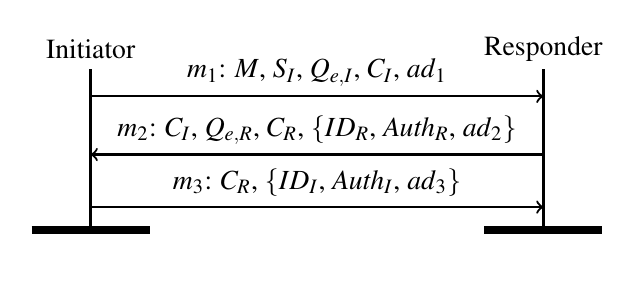
\begin{tikzpicture}
    \node (ini) at (0, 0) {Initiator};
    \draw [very thick] (0, -0.25) -- (0,-2.3);
    \draw [very thick] (5.75, -0.25) -- (5.75,-2.3);
    \node (res) at (5.75,0) {Responder};
    \msg{1em}{ini}{res}{\mMsgone: \mMethod, \mSuites, \mGx, \mCi, \mADone};
    \msg{3em}{res}{ini}{\mMsgtwo: \mCi, \mGy, \mCr, \{\mIdcredr, \mAuthr, \mADtwo\}};
    \msg{5em}{ini}{res}{\mMsgthree: \mCr, \{\mIdcredi, \mAuthi, \mADthree\}};
    \draw [line width=1mm] (-0.75,-2.3) -- (0.75,-2.3);
    \draw [line width=1mm] (5.75-0.75,-2.3) -- (5.75+0.75,-2.3);
    \node (padding) at (0,-2.5) {};
    \end{tikzpicture}
    \caption{Structure of \mEdhoc{}: $\{t\}$ means $t$ is encrypted and integrity
protected.~\cite{Norr21}}
\label{fig:edhocFramework}
\end{figure}
%
Of the three messages, the first two, among other things, serve to establish a
common authentication method \mMethod{}, and a ciphersuite \mSuites{}.
%
In \mMethod{}, the party playing the initiator role proposes which
authentication methods the two parties shall use, and an ordered list
of choices for the ciphersuite.
%
As mentioned earlier, the authentication methods may differ for the two roles,
yielding four possible
combinations: \mSigSig{}, \mSigStat{}, \mStatSig{}, and \mStatStat{},
where the first authentication method in each combination is used by the
initiator role, and the second by the responder role.
\footnote{As in the \mSpec{}, we will from now on overload
notation and refer to the combinations of authentication methods as methods as
well.}
%
The party executing the responder role may choose to reject the method or
ciphersuite chosen by the initiator by sending an error message.
%
This results in abandoning this session and renegotiating, as the initiator
goes down their list of choices for ciphersuites, and picks the next option for
a next execution of the protocol.
%
Our analysis does not cover such renegotiation which requires maintaining state
between executions to remember the rejected ciphersuites.
%
However, we will discuss the ramifications of such a renegotiation procedure
and the error messages later, in Section~\ref{sec:}.
%

In addition to negotiating the ciphersuite, the first two messages are
also instrumental for the exchange of public ephemeral keys \mGx{} and \mGy{},
and connection identifiers \mCi{} and \mCr{}, for the initiator and responder
roles respectively.
%
The \mSpec{} states that the connection identifiers serve only to route messages
to the correct party executing \mEdhoc{}, but also claims that they may be
used in turn by protocols (like \mOscore{}) using the security context
established by \mEdhoc{}.
%
While the \mSpec{} does not require any explicit security guarantees to be
satisfied by these connection identifiers, it does, however, require that the
identifiers be unique, i.e., in any session, $\mCi{} \neq \mCr{}$, and that the
parties involved in the session can verify this uniqueness.
%
More precisely, the \mSpec{} states that \mOscore{} should be able to use these
identifiers to retrieve any particular security context.
%
In this work, as in~\cite{Norr21}, we verify that the parties agree on the
values of \mCi{} and \mCr{}.
%
The second and third messages also serve to identify and authenticate each
party to the other.
%
These messages contain long-term key identifiers (\mIdcredi{} and \mIdcredr{}).
%
Additionally, the messages contain authenticating information
(\mAuthi{} and \mAuthr{}), which lets each
party know that the other party does indeed control the long-term key
associated with these identifiers.
%
The authentication information is different for each authentication method.
%
Consider the following example scenario.
%
The initiator $I$ chooses the method $\mSigStat{}$ and sends this via
$\mMethod{}$ to the responder $R$.
%
$R$ now has an option to either reject this choice of method, or to provide an
identifier \mIdcredr{} for a key pair which can be used with challenge-response
signatures as well as authenticating information \mAuthr{}, as dictated by
the static key authentication method \mStat{}.
%
$I$ will then respond with an identifier \mIdcredi{} corresponding to a key
pair, which is suitable for regular signatures, and provide authentication
\mAuthi{} as appropriate for the signature-based method \mSig{}.

%-------------------------------------------------------------------------- sub
\subsection{Key Schedule}
\label{sec:keysched}
As mentioned above, the second and third messages of \mEdhoc{} contain
authenticating information.
%
This information is either a signature or a message authentication code (MAC),
as we will describe in more detail in Section~\ref{sec:edhocauth}.
%
The keys for these are generated by using a key schedule which takes at least
one DH key \mGxy{} as basic input, as shown in Figure~\ref{fig:kdfdiagram},
and is intrinsic to the functioning of \mEdhoc{}.
%
\begin{figure}[!h]
\scalebox{.785}{
% !TEX root =  protocol.tex

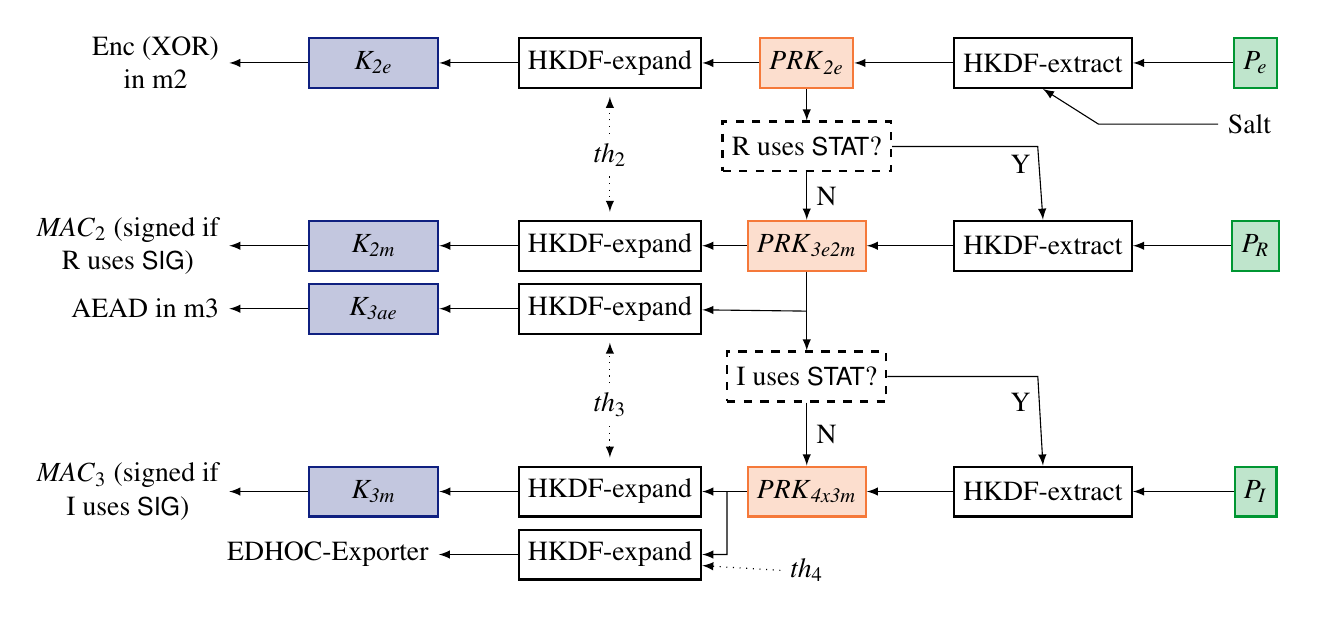
\begin{tikzpicture}[%
    >=latex,              % Nice arrows; your taste may be different
    start chain=going below,    % General flow is top-to-bottom
    node distance=4mm and 60mm, % Global setup of box spacing
    every join/.style={norm},   % Default linetype for connecting boxes
    ]
% ------------------------------------------------- 
% A few box styles 
% <on chain> *and* <on grid> reduce the need for manual relative
% positioning of nodes
\tikzset{
terminput/.style={rounded corners},
term/.style={rounded corners},
  base/.style={draw, thick, on chain, on grid, align=center, minimum height=4ex},
  dhkbox/.style={draw=cbgreen, fill=cbgreen!25, rectangle},
  dhk/.style={base, dhkbox},
  prkbox/.style={draw=cborange, fill=cborange!25, rectangle},
  prk/.style={base, prkbox},
  %hkdfext/.style={base, draw=Green3, fill=Green3!25, isosceles triangle, isosceles triangle apex angle=60, anchor=base, shape border rotate=-90, text width=6em},
  hkdfext/.style={base, draw=black, fill=none, rectangle},
  %hkdfexp/.style={base, draw=orange, fill=orange!50, isosceles triangle, isosceles triangle apex angle=60, anchor=base, shape border rotate=-90, text width=6em},
  hkdfexp/.style={base, draw=black, fill=none, rectangle},
  keybbox/.style={draw=cbnavy, fill=cbnavy!25, rectangle},
  keyb/.style={base, keybbox, text width=4em},
  % -------------------------------------------------
  norm/.style={->, draw, black},
  cond/.style={base, draw=black, dashed, fill=none, rectangle},
  txt/.style={base, draw=none, fill=none}
  }
% -------------------------------------------------
% Start by placing the nodes
%\node [terminput] (u1) {Salt};
%\node [hkdfext, join] (h1) {\mHkdfExtract};
\node [prk, join] (p2) {\mPRKtwo};
\node [cond, join] (c1) {R uses \mStat?};

\node [prk, below=6mm of c1.south] (p3) {\mPRKthree};
\draw [->, norm] (c1.south) -- (p3.north) node[midway, right] {N};

\node [cond, join, below=10mm of p3.south] (c2) {I uses \mStat?};
\node [prk, below=8mm of c2.south] (p4) {\mPRKfour};
\draw [->, norm] (c2.south) -- (p4.north) node[midway, right] {N};

\node [hkdfext, right=3cm of p3] (h3) {\mHkdfExtract};
\node [hkdfext, right=3cm of p4] (h5) {\mHkdfExtract};

\node [hkdfexp, shape border rotate=180, left= 2.5cm of p4] (h6) {\mHkdfExpand};
\node [keyb, join, left=3cm of h6] (k3) {\mKthreem};
\node [hkdfexp, shape border rotate=180, below= 0.8cm of h6] (h9) {\mHkdfExpand};
\node [txt, join, left=1cm of h9.west] (t4) {EDHOC-Exporter};

\node [hkdfexp, shape border rotate=180, left= 2.5cm of p3] (h4) {\mHkdfExpand};
\node [keyb, join, left=3cm of h4] (k2) {\mKtwom};

\node [hkdfexp, shape border rotate=180, left= 2.5cm of p2] (h2) {\mHkdfExpand};
\node [keyb, join, left=3cm of h2] (k1) {\mKtwoe};

\node [hkdfexp, shape border rotate=180, below= 0.8cm of h4] (h8) {\mHkdfExpand};
\node [keyb, below=0.8cm of k2] (k2b) {\mKthreeae};

\node [txt, left=1cm of k1.west] (t1) {Enc (XOR) \\ in m2};
\node [txt, left=1cm of k2.west] (t2) {\mMactwo~(signed if \\ R uses \mSig)};
\node [txt, left=1cm of k2b.west] (t2b) {\mAead\ in m3};
\node [txt, left=1cm of k3.west] (t3) {\mMacthree~(signed if \\ I uses \mSig)};

\draw [->, norm] (k1.west) -- (t1.east);
\draw [->, norm] (k2.west) -- (t2.east);
\draw [->, norm] (k2b.west) -- (t2b.east);
\draw [->, norm] (k3.west) -- (t3.east);

\draw [->, norm] (p3.south) ++(0,-0.5) -- (h8);
\draw [->, norm] (h8) -- (k2b);
\draw [->, norm] (p2) -- (h2); 
\draw [->, norm] (c1.east) -- ++(1.85,0) -- (h3.north) node[midway,above left] {Y};
%\draw [->, norm] (h3.south) -- ++(0,-1) -- ++(-3,0);
\draw [->, norm] (h3.west) -- (p3.east);
\draw [->, norm] (p3) -- (h4); 
\draw [->, norm] (c2.east) -- ++(1.91,0) -- (h5.north) node[midway,above left] {Y};
%\draw [->, norm] (h5.south) -- ++(0,-1) -- ++(-3,0);
\draw [->, norm] (h5.west) -- (p4.east);
\draw [->, norm] (p4) -- (h6);
\draw [->, norm] (p4.west) ++(-0.25,-0) -- ++(0,-0.8) -- (h9.east);

\node [hkdfext, right=3cm of p2] (h1) {\mHkdfExtract};
\node [dhk, right=2.7cm of h1] (p0) {$\mGxy$};
\node [terminput, text width=2em, below = 0.2cm of p0] (u1) {Salt};
\draw [->] (h1.west) -- (p2.east);
\draw [->] (u1.west) -- ++(-1.52,0) -- (h1.south);
\draw [->] (p0.west) -- (h1.east);


\node [dhk, right = 2.7cm of h3] (u2) {$P_R$};
\draw [->, norm] (u2.west) -- (h3.east);

\node [dhk, right = 2.7cm of h5] (u3) {$P_I$};
\draw [->, norm] (u3.west) -- (h5.east);


\node [term, above = 0.55cm of h4] (u5) {\mTHtwo};
\draw [->, dotted, shorten >=1mm] (u5) -- (h4);
\draw [->, dotted, shorten >=1mm] (u5) -- (h2);

\node [term, above = 0.5cm of h6] (u6) {\mTHthree};
\draw [->, dotted, shorten >=1mm] (u6) -- (h6);
\draw [->, dotted, shorten >=1mm] (u6) -- (h8);

%\node [term, below= 1cm of h9] (u7) {\mTHfour};
\node [term, below=0.4cm of p4] (u7) {\mTHfour};
%\draw [->, dotted, shorten >=1mm] (u7) -- (h9.south);
\draw [-> , dotted ] (u7.west) -- ([yshift=-0.4em] h9.east);

%\matrix [draw, ultra thick, double, below=2em of t1.east] {
%  \node [dhkbox, semithick, label=right:DH key] {}; \\
%  \node [prkbox, semithick, label=right:Intermediate key material] {}; \\
%  \node [keybbox, semithick, label=right:Key for \mAead{} or \mXor] {}; \\
%};

%
% ------------------------------------------------- 
% 
%\path (h2.east) to node [near start, yshift=1em] {$n$} (c3); 
%  \draw [o->,lccong] (h2.east) -- (p8);
%\path (p3.east) to node [yshift=-1em] {$k \leq 0$} (c4r); 
%  \draw [o->,lcnorm] (p3.east) -- (p9);
% -------------------------------------------------
% A last flourish which breaks all the rules
%\draw [->,MediumPurple4, dotted, thick, shorten >=1mm]
%  (p9.south) -- ++(5mm,-3mm)  -- ++(27mm,0) 
%  |- node [black, near end, yshift=0.75em, it]
%    {(When message + resources available)} (p0);
% -------------------------------------------------
\end{tikzpicture}


}
\caption{Key schedule: $P_e, P_I, P_R$ are the DH keys, \mPRKtwo, \mPRKthree, \mPRKfour{} are the intermediate key material, and \mKtwoe,\mKtwom, \mKthreeae, \mKthreem{} are the encryption keys for \mAead{} or \mXor{}. Dashed boxes are conditionals.~\cite{Norr21}}
\label{fig:kdfdiagram}
\end{figure}
%

To derive keys, \mEdhoc{} uses two functions from the \mHkdf{}
interface~\cite{rfc5869}, \mHkdfExtract{} and \mHkdfExpand{}.
%
Both functions take as argument two values -- a salt, and an input.
%
For \mHkdfExtract{}, the input is a DH key, while for \mHkdfExpand{},
it is intermediate key material.
%

As mentioned earlier, the fundamental building block for the key schedule is
the ephemeral DH key \mGxy{}, which is computed in two different ways by
$I$ (as $\mDH(\mX, \mGy)$) and $R$ (as $\mDH(\mY, \mGx)$).
%
This key gives rise to intermediate keys \mPRKtwo{}, \mPRKthree{} and
\mPRKfour{}, which can be derived as part of protocol execution.
%
Each intermediate key gives rise to encryption and integrity keys
(\mKtwoe, \mKtwom{}, \mKthreeae, and \mKthreem)
for a particular message in the protocol.
%

In order to generate the final keys, the two \mHkdf{} algorithms use various
values for salt.
%
\mPRKtwo{} is generated by the \mHkdfExtract{} algorithm while using the empty
string as the salt.
%
\mPRKthree{} and \mPRKfour{} are separately generated if $R$ or $I$ uses the
\mStat{} method, using the corresponding DH key as input and the previous
intermediate key as salt.
%
The key $P_{R}$ is used if the responder uses the \mStat{} authentication method.
%
$P_{R}$ is the key computed as $\mDH(\mX,\ \mGr{}) = \mDH(\mPriv{R},\ \mGx)$.
%
Similarly, the key $P_{I}$ is used if the initiator uses \mStat{}, and is computed as $\mDH(\mY,\ \mGi{}) = \mDH(\mPriv{I},\ \mGy)$.
%

These intermediate keys are fed into \mHkdfExpand{}, as shown in Figure~\ref{fig:kdfdiagram}.
%
\mHkdfExpand{} here uses as salt a value $\textit{th}$, which is a running hash of the information transmitted thus far as part of the protocol.
%
$\textit{th}_{i}$ denotes the hash corresponding to the $i^{\rm{th}}$ message.
%

At the end of a successful run of the protocol, the session key material is
established as \mSessKey{}, which we define as a set of various keys.
%
This set always includes \mGxy{}, and if the initiator (resp. the responder) uses the \mStat{} authentication method, then it also includes $P_{I}$ (resp. $P_{R}$).
%
We discuss which material should be included in \mSessKey{} in more detail in
the formal model in Section~\ref{sec:formalization} and the consequences of
various choices in Section~\ref{sec:sessionKeyMaterial}.
%
Once \mSessKey{} has been established, an \mHkdf{}-based key exporter named
\mEdhoc-Exporter extracts the keys required by the security protocol.
%

%-------------------------------------------------------------------------- sub
\subsection{About Authentication in \mEdhoc{}}
\label{sec:edhocauth}
We now describe how the authentication information is constructed, depending on which method is used.
%
For both \mStat{} and \mSig{}, the following information is used to compute
\mAuthr{}: \mIdcredr{}, \mCredr{}, a transcript hash of all the communicated
information thus far in the protocol, and \mADtwo{}, if included.
%
\mAuthi{} uses the same pieces of information, but corresponding to the
initiator role.
%
A MAC is obtained by feeding this material as additional data and the empty
string as input to the Authenticated Encryption with Additional Data (AEAD)
encryption algorithm as indicated in the established ciphersuite \mSuites{}.
%
The encryption key for the AEAD algorithm is constructed, for both roles,
using the ephemeral key material \mGx{}, \mGy{}, \mX{}, and \mY{}.
%
The initiator computes $\mDH(\mX, \mGy)$ while the responder computes
$\mDH(\mY, \mGx)$, and DH operations give rise to the same key under both
these computations.
%

When $I$ uses the \mSig{} authentication method, \mAuthi{} is $I$'s signature
over the MAC along with the data covered by the MAC.
%
However, when $I$ uses the \mStat{} method, \mAuthi{} is just the MAC, with
one difference: the MAC key is derived using both the ephemeral key material
\mGxy{} as well as the long-term key for the initiator
$\langle\mPriv{I},\ \mPub{I}\rangle$.
%
This is similar to the 1-RTT semi-static pattern in \mOptls which computes the
MAC key \textsf{sfk} for the message
\textsf{sfin}~\cite{DBLP:conf/eurosp/KrawczykW16}.
%
The same procedures works for $R$ as well (with the values corresponding to $R$).
%
The abstract calculation for the authentication information values is as shown
in Table~\ref{tab:authvalues}~\cite{Norr21}.
%
We use $\mathit{MAC}_{I}$ (resp. $\mathit{MAC}_{R}$) to denote a MAC which uses
an encryption key constructed using
$\langle\mPriv{R},\ \mPub{R}\rangle$ and $\langle\mX,\ \mGx\rangle$
(resp. using $\langle\mPriv{I},\ \mPub{I}\rangle$ and $\langle\mY,\ \mGy\rangle$).
%
\begin{table}[ht]
\centering
\begin{tabular}{|c|c|c|}
        \hline
        \mMethod & \mAuthi & \mAuthr\\
        \hline
        \mSigSig{} & $\mSign{I}(\cdot)$ & $\mSign{R}(\cdot)$ \\
        \mSigStat{} & $\mSign{I}(\cdot)$ & $\textit{MAC}_R(\cdot)$\\
        \mStatSig{} & $\textit{MAC}_I(\cdot)$ & $\mSign{R}(\cdot)$\\
        \mStatStat{} & $\textit{MAC}_I(\cdot)$ & $\textit{MAC}_R(\cdot)$\\
        \hline
\end{tabular}
\caption{The outer functions for each method \mMethod{}~\cite{Norr21}}
\label{tab:authvalues}
\end{table}
%

In addition to this, the second and third messages have
provisions for transferring application messages which are encrypted and
integrity protected, as can be seen in~\ref{fig:edhocFramework}.
%
The second message is encrypted by performing a bit-wise \mXor{} between
the plaintext and the output of the key derivation function \mHkdf{}, as
in Section~\ref{sec:keysched}.
%
For the third message, encryption and integrity protection is assured by the
\mAead{} algorithm which is part of the established ciphersuite \mSuites{}.
%

In Figure~\ref{fig:edhocsigstat} we show an example of protocol execution under
the \mSigStat{} method.
%
The figure describes in detail the various message patterns, operations and
key derivations used to construct these messages.
%\vnote{Do we still have the other method diagrams that we wrote out for the original paper but did not include?}
%\knote{I don't think we have space for that.}
%
\begin{figure}[ht]
\centering
\scalebox{.7}{
\tikzset{>=latex, every msg/.style={draw=thick}, every node/.style={fill=none,text=black}}
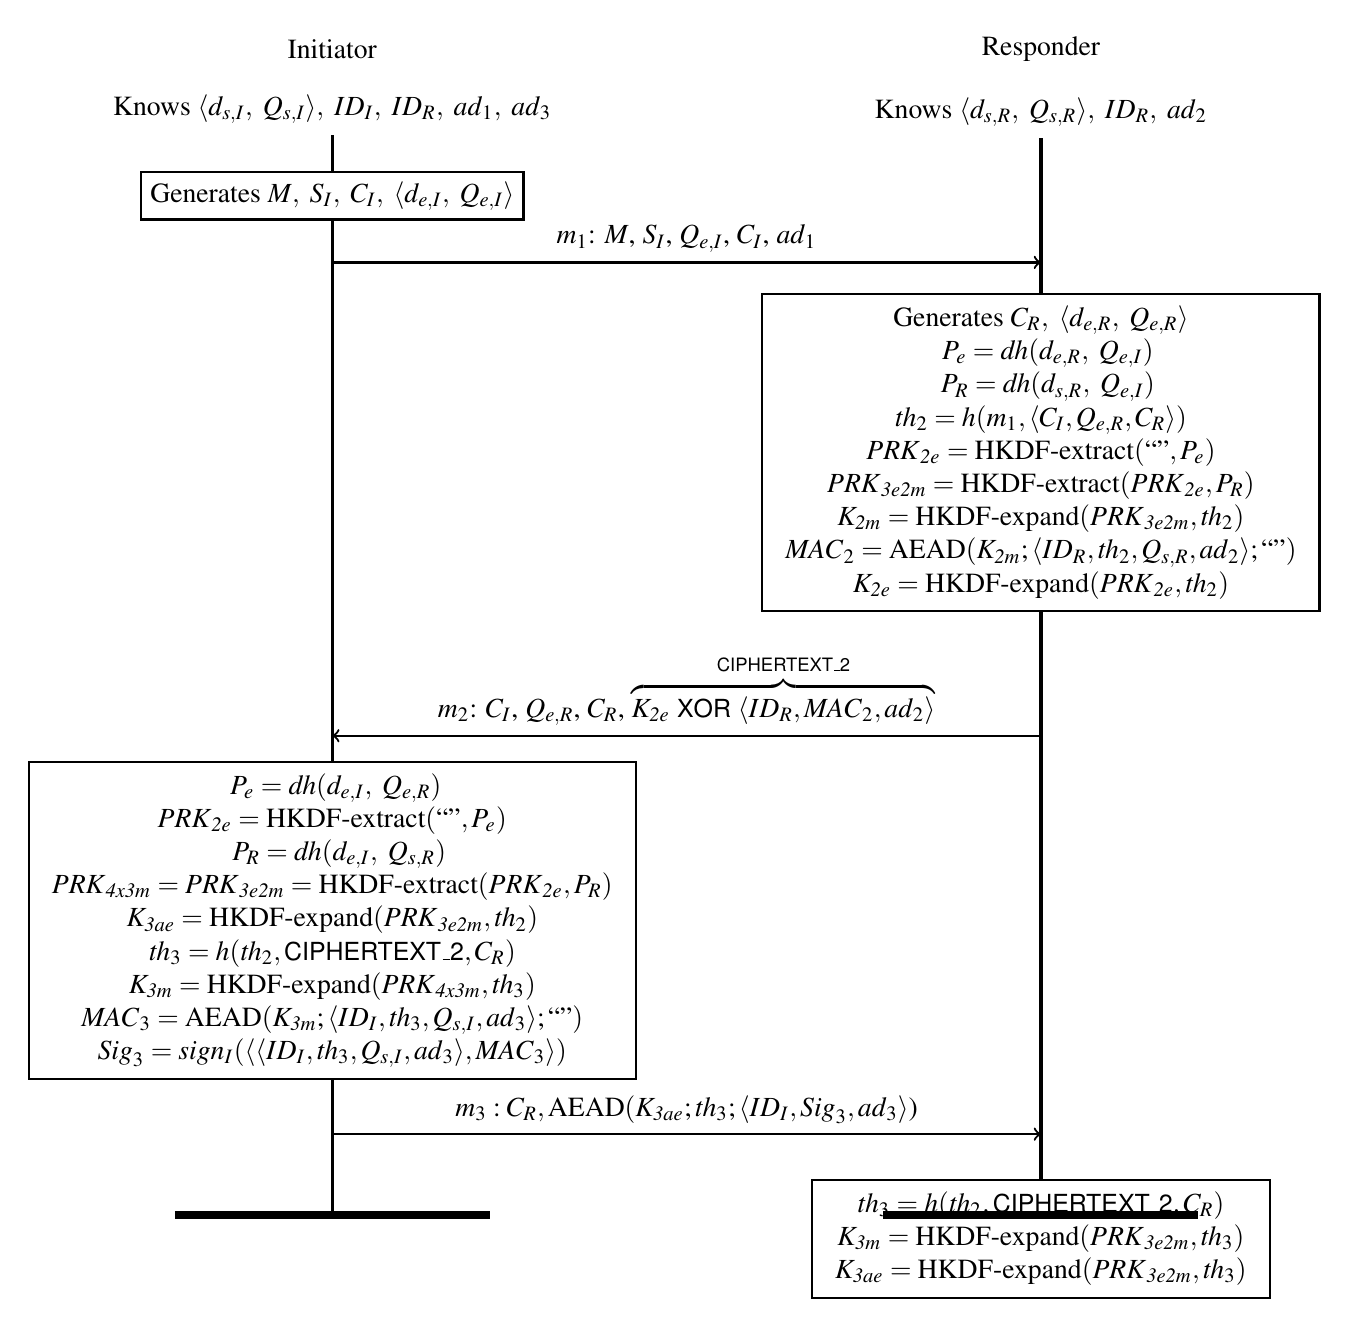
\begin{tikzpicture}
    \node (ini) at (0, 0) {Initiator};
    \draw [very thick] (0, -0.5) -- (0,-14.8);
    \draw [very thick] (9, -0.5) -- (9,-14.8);
    \node[below=0.5em of ini,fill=white] {$
    \begin{array}{c}
        \text{Knows}\ \langle\mPriv{I},\ \mPub{I}\rangle,\ \mIdcredi,\ \mIdcredr,\ \mADone,\ \mADthree
    \end{array}
    $};
    \node (res) at (9,0) {Responder};
    \node[below=0.5em of res,fill=white] {$
    \begin{array}{c}
        \text{Knows}\ \langle\mPriv{R},\ \mPub{R}\rangle, \ \mIdcredr,\ \mADtwo
    \end{array}$};
    \action{3.7em}{ini}{Generates $\mMethod,\ \mSuites,\ \mCi,\ \langle\mX{},\ \mGx\rangle$};
    \msg{7em}{ini}{res}{\mMsgone: \mMethod, \mSuites, \mGx, \mCi, \mADone};
    \action{8em}{res}{$
      \begin{array}{c}
          \text{Generates } \mCr,\ \langle\mY{},\ \mGy\rangle\\
          \ \ P_e = \mDH(\mY,\ \mGx{})\\
          \ \ P_R = \mDH(\mPriv{R},\ \mGx{})\\
        \mTHtwo = \mHash(\mMsgone, \langle \mCi, \mGy, \mCr \rangle)\\
        \mPRKtwo = \mHkdfExtract(\textrm{``\phantom{}''}, P_e) \\
        \mPRKthree = \mHkdfExtract(\mPRKtwo, P_R) \\
        \mKtwom = \mHkdfExpand(\mPRKthree, \mTHtwo) \\
        \mMactwo = \mAead(\mKtwom; \langle \mIdcredr, \mTHtwo, \mCredr, \mADtwo \rangle; \textrm{``\phantom{}''}) \\
        \mKtwoe = \mHkdfExpand(\mPRKtwo, \mTHtwo)
      \end{array}$};
    \msg{24em}{res}{ini}{\mMsgtwo: \mCi, \mGy, \mCr, $\overbrace{\mKtwoe\ \mXor\ \langle \mIdcredr, \mMactwo, \mADtwo \rangle}^{\mCipher}$};
    \action{25em}{ini}{$
      \begin{array}{c}
        %\mTHtwo = \mHash(\mMsgone, \langle \mCi, \mGy, \mCr \rangle) \
        \ P_e = \mDH(\mX,\ \mGy{})\\
        \mPRKtwo = \mHkdfExtract(\textrm{``\phantom{}''}, P_e) \\
        %\mKtwoe = \mHkdfExpand(\mPRKtwo,\mTHtwo)\\
        %\mGrx = \mCredr^{x} \\
        \ \ P_R = \mDH(\mX,\ \mPub{R})\\
        \mPRKfour = \mPRKthree = \mHkdfExtract(\mPRKtwo, P_R) \\
        %\mKtwom = \mHkdfExpand(\mPRKthree, \mTHtwo) \\
        \mKthreeae = \mHkdfExpand(\mPRKthree, \mTHtwo) \\
        \mTHthree = \mHash(\mTHtwo, \mCipher, \mCr)\\
        \mKthreem = \mHkdfExpand(\mPRKfour, \mTHthree) \\
        \mMacthree = \mAead(\mKthreem; \langle \mIdcredi, \mTHthree, \mCredi, \mADthree \rangle; \textrm{``\phantom{}''}) \\
        \mSigthree = \mSign{I}(\langle \langle \mIdcredi, \mTHthree, \mCredi, \mADthree \rangle, \mMacthree \rangle)
      \end{array}$};
    \msg{38.5em}{ini}{res}{$\mMsgthree: \mCr, \mAead(\mKthreeae; \mTHthree; \langle \mIdcredi, \mSigthree, \mADthree \rangle$)};
    \action{40em}{res}{$
    \begin{array}{c}
        \mTHthree = \mHash(\mTHtwo, \mCipher, \mCr)\\
        \mKthreem = \mHkdfExpand(\mPRKthree, \mTHthree) \\
        \mKthreeae = \mHkdfExpand(\mPRKthree, \mTHthree)
    \end{array}$};
    \draw [line width=1mm] (-2,-14.8) -- (2,-14.8);
    \draw [line width=1mm] (7,-14.8) -- (11,-14.8);
    \end{tikzpicture}
}
    \caption{The \mSigStat{} method for \mEdhoc{}. $\langle\cdot\rangle$ denotes a tuple, and the hash function \mHash{} is as established in the ciphersuite \mSuites{}.~\cite{Norr21}}
\label{fig:edhocsigstat}
\end{figure}

%------------------------------------------------------------------------- sec
\section{Implementation Aspects and Key Protection}
\label{sec:TEE}
Authentication of a specific IoT device assumes that this devices is the only
entity with access to the long-term key associated with the corresponding
identity.
%
Since IoT devices may be accessible to adversaries, e.g., an insider cloning a
key card, the long-term keys must be appropriately protected.
%
A state of the art approach is to use a Trusted Execution Environment (TEE),
which holds the key and provides an API for operations using the key.
%
This is the approach taken by the
Trust-Zone based \mMuEdhoc{}~\cite{DBLP:conf/codaspy/Hristozov0XFLS21}
implementation for example.
%
Typical operations include signatures using the long-term private key of a
party.
%

TEEs come in various forms of differing complexity.
%
Some, like ARM Trust Zone and Intel SGX are general purpose execution
environments, which are flexibly programmable.
%
Other, like the Universal Subscriber Identity Modules (USIM) used for
authentication to 3GPP mobile networks, have application specific interfaces for
authentication and key agreement protocols etc.
%
A key aspect is how much of the application is placed in the TEE and how much is
outside.
%

For larger devices that include general purpose processors with Trust Zone or
SGX, entire \mEdhoc{} and \mOscore{} may reside inside the TEE.
%
For constrained IoT devices in the lower end of the scale, a TEE may have to be
implemented using a special-purpose integrated circuit.
%
In the latter case, it may be beneficial to follow a minimalistic approach, and
contain the long-term key and only
the operations that need access to it in the TEE for cost reasons.
%

It may at first appear more secure to implement as much as possible inside the
TEE, but there is a security trade-off: the more code inside the TEE,
the higher the risk of implementation errors in the security-critical code.
%
Because the security critical code runs in the area where the long-term keys
reside, an implementation error here risks leaking information of the key to the
adversary.
%
From this perspective, it may be beneficial to follow the minimalistic approach
even when having access to Trust Zone or SGX.
%

A slightly more secure division of functionality is to also keep the
session key inside
the TEE and extend the interface to accept messages and return the
(en/de)crypted counter part.
%
That is, the interface exposes \mAead{} functions in the interface.
%



%-------------------------------------------------------------------------- sec
\section{\uppercase{Formalization and Results}}
\label{sec:formalization}
% !TEX root = paper.tex
The \mEdhoc{} \mSpec{} \cite{our-analysis-selander-lake-edhoc-00} claims
that \mEdhoc{} satisfies many security properties, but these are imprecisely
expressed and motivated.
%
In particular, there is no coherent adversary model.
%
It is therefore not clear in which context properties should be verified.
%
We resolve this by clearly specifying an adversary model, in which we can 
verify
properties.
%

\subsection{Formal Model}\label{sec:threat-model}
As in~\cite{Norr21}, we verify \mEdhoc{} in an extended
Dolev-Yao model~\cite{DY83}.
%
Dolev-Yao is a well-established model for symbolic verification of security
protocols.
%
Messages are modelled as terms in an algebra, and the various cryptographic
operations are assumed to be perfect, e.g., encrypted messages can only be
decrypted with the correct key, and there are no hash collisions.
%

The adversary is assumed to be in control of the communication
channel and can see all messages being communicated as part of the protocol.
%
In addition, they can interact with an unbounded number of protocol sessions,
drop, inject and modify messages at will.
%

On top of the standard Dolev-Yao model,~\cite{Norr21} allows the adversary to
access the long-term and ephemeral keys.
%
Long-term key reveal, denoted $\mRevLTK^{t}(A)$, stands for the adversary
gaining access to a party $A$'s long-term private key \mPriv{A} at a time point $t$.
%
Ephemeral key reveal, denoted $\mRevEph^{t}(A, k)$, stands for the adversary
obtaining, at time $t$, the ephemeral private key \mPrivE{A} used by party $A$
in a session where they establish key material $k$.
%
Formalizing these two capabilities allows more fine-grained control
over the access that an adversary has to these fundamentally different kinds of
keys.
%
Furthermore, we extend the results from~\cite{Norr21} by strengthening the
adversary capabilities, as detailed next.
%

%---------------------------------------------------------------------- subsub
\subsubsection{System and Adversary Model Extensions Supporting TEE.}
\label{sec:TEE:advModel}
%
We extend the adversary model of~\cite{Norr21} by introducing an interface to
allow the adversary to use the long term key material of any party, though
without directly accessing such key material.
%
This allows us to model the scenario where the adversary has gained access to
a device, but the long term key material is protected by a trusted execution
environment (TEE), and thus only accessible through the TEE interface.
%
According to the terminology of~\cite{DBLP:conf/csfw/Cohn-GordonCG16}, a
protocol is considered to have \emph{weak post-compromise security}
(Weak-PCS) if it achieves its security goals for a specific session
even when the attacker has limited access to the long-term key material
of the parties involved before the session starts -- through an interface 
that maintains the key material secure but allows to run cryptographic 
operations with it -- and full access to the key material of the parties
involved after the end of the session, as well as access to the key material
of all other parties.
%
Seen in the framework of~\cite{DBLP:conf/icics/XuZRWTZ20}, we add adversary
capabilities corresponding to a server adversary, i.e., an adversary that
compromises a party, learns its ephemeral keys and may temporarily access its
TEE, but does not learn the party's long-term key.
%
Our extension to the model of~\cite{Norr21} thus allows us to verify all the
previous security properties under a Weak-PCS model.
%
Note that this attacker model is strictly more powerful than that of~\cite{Norr21},
as it maintains all the previous attacker capabilities.
%

We split the \mEdhoc{} functionality as follows.
%
The TEE contains the long-term key and allows the non-TEE parts of the
application to perform the operations on it via its interface.
%
More precisely, parties using the \mSig{} authentication method use a TEE 
with an interface which accepts a message and returns the signature of that 
message using the party's private long-term key.
%
A party $U$ using the \mStat{} authentication method use a TEE with an 
interface accepting a point $P$ on the curve and returning $\mDH(P,\ \mGu{})$.
%

The non-TEE parts implement \mEdhoc{} using this interface.
%
This interface requires the least functionality from the TEE, reducing the 
TEE's complexity and possibly cost of its implementation.
%
This functional split is suitable even when a constrained device has
implemented only the storage of the long-term key in 
a special purpose circuit with minimal processing functionality.
%
Since \mEdhoc{} focuses on constrained IoT devices, it seems appropriate to
cater for this setting.
%

%---------------------------------------------------------------------- subsub
\subsubsection{Extended Formalism and Security Properties.}
\label{sec:TEE:fmAndProps}
Formally, we model the TEE interface by adding two new rewrite rules:
%
\begin{small}
\begin{verbatim}
rule forge_SIG:
   [!LTK_SIG($A, ~ltk), In(xx)] --[TEE($A)]-> [Out(sign(xx, ~ltk))]

rule exp_STAT:
   [!LTK_STAT($A, ~ltk), In('g'^~xx)] --[TEE($A)]-> [Out(('g'^~xx)^~ltk)]
\end{verbatim}
\end{small}
%
These rules allow the adversary to obtain terms representing signatures on a
value of their choice to forge signatures (\verb|forge_SIG|), or to obtain terms
representing a curve point of their choice raised to the power of the
long-term key (\verb|exp_STAT|).
%

Because it is a trivial attack when the adversary access these rules with values
from the test session, we must disqualify those rule applications.
%
We do so by creating an action fact \verb|TEE($A)|, where \verb|$A| is the
identity corresponding to the private key used, and then augmenting the
properties with a condition that no such action fact exists from the start of
the protocol execution and its end.
%
Care must be taken when specifying the start and the end: specifically,
the start and end of the protocol run must be viewed w.r.t. the current
role.
%
For example, the injective agreement property for the initiator in
the \mSigSig{} method requires that the adversary does not have access to the
TEE of the responder from the time of transmission of the first message until
the second message is received by the initiator.
%
Because reception of one message and transmission of the next one at a party
is an atomic operation, these timepoints represent the start and end of the
protocol run from the perspective of the initiator.
%

With this additional attacker capability Tamarin manages to prove
almost all lemmas and method combinations, except for the implicit
authentication lemmas when the responder uses the \mStat{} authentication
method: in these two cases Tamarin did not complete the within reasonable
time\footnote{See Table~\ref{tab:props} for all verification results and
computation times.}.
%
We therefore simplified the modeling of XOR encryption of the second
message to prove implicit authentication when the responder uses the 
\mStat{} method.
%
More precisely, the second message encrypts two values: the responder's identity
\verb|R| and the authentication information \verb|authR|.
%
We model XOR encryption by xor-ing each term with their own key-stream term.
%
However for the problematic cases we xor the entire tuple
\verb|<R, authR>| with a single key-stream term.
%
This simplification might miss an attack on implicit authentication that is due
to the combination of a malleable XOR encryption and access to the TEE interface.
%
However, given that no attacks were identified using our original modeling due
to the use of XOR, nor in the current modeling for all other authentication 
methods, we believe that this is not a severe restriction.
%

Next we describe \mTamarin{}, and our modeling of \mEdhoc{}.
%

%-------------------------------------------------------------------------- sub
\subsection{\mTamarin{}}
\label{sec:tamarin}
We extend the formal \mEdhoc{} model of~\cite{Norr21}, using the symbolic
model tool \mTamarin{}~\cite{DBLP:conf/cav/MeierSCB13}, which is an 
interactive
tool for the formal verification of security protocols.
%
Protocols are modelled in \mTamarin{} as multiset rewrite rules which encode 
a
transition relation.
%
The elements of these multisets, called facts, contribute to the global
system state.
%
For syntactic sugar, \mTamarin{} also allows the use of let-bindings and tuples.
%
For ease of presentation, we will present the model and properties in a
slightly different syntax in this paper, but this syntax can be directly
mapped to that of \mTamarin.
%

Rewrite rules can be annotated with events, called actions in \mTamarin{}.
%
Communicated messages in the protocol are modelled as terms in an algebra,
which specifies sets of names, variables, and allowable function symbols.
%
Facts and actions are modelled as $n$-ary predicates in the term algebra,
and actions can be parametrized using terms.
%

An annotated multiset rewrite-rule is represented as
$l \ifarrow[e] r$, where $l$ and $r$ are multisets, and $e$ is
a multiset of actions.
%
A sequence of actions yields a protocol execution trace.
%
Event types are predicates over global states generated during protocol 
execution.
%
Consider an event type $E$ and a timestamp $t$ as part of a trace.
%
By $E^{t}(p_i)_{i\in\mathbb{N}}$, we represent an event of type $E$ occurring
at time $t$ in a trace, parametrized by the sequence of values
$(p_i)_{i\in\mathbb{N}}$
(corresponding to the action fact $E(p_i)_{i\in\mathbb{N}}@t$ in \mTamarin).
%
Thus, the time points form a quasi order, and we denote the fact that
$t_{1}$ comes before $t_{2}$ in a protocol trace by
$t_{1} \lessdot t_{2}$, and that $t_{1}$ and $t_{2}$ stand for the same
time point in a trace by $t_{1} \doteq t_{2}$.
%
\mTamarin{} allows events to occur at the same time point, with one
restriction: multiple events of the same type cannot occur simultaneously,
so if $t_{1} \doteq t_{2}$, then $E^{t_{1}} = E^{t_{2}}$.
%

Properties are defined as formulas in a fragment of temporal first order logic,
and these formulas can be verified over execution traces.
%

Protocol verification in \mTamarin{} happens under an equational theory $E$.
%
For example, to represent the fact that $E$ satisfies the reversal of
symmetric encryption by using a decryption operation with the key,
one can write $\textit{dec}(\textit{enc}(x, y), y) =_{E} x$.
%
The equational theory $E$ is fixed upfront to handle the functions supported 
by
the term algebra, so we will omit the subscript for the rest of this paper.
%

Users can extend the default term algebra and equational theory in
\mTamarin{} with new function symbols and unification rules for these new 
symbols.
%
For example, \mEdhoc{} requires authenticated encryption, which we model 
using
the symbol \mT{aeadEncrypt}.
%
We augment \mTamarin{} with the following rule for this operation,
which represents the fact that if the adversary knows a key \mT{k},
a message \mT{m}, and authenticated data \mT{ad},
and has access to an encryption algorithm \mT{ai},
then they can obtain the message corresponding to the authenticated 
encryption
of \mT{m} with \mT{k}~\cite{Norr21}.
%
{\footnotesize
\begin{verbatim}
[!KU(k), !KU(m), !KU(ad), !KU(ai)] --[]-> [!KU(aeadEncrypt(k, m, ad, ai))]
\end{verbatim}}
%
Other than modeling authenticated encryption, we use \mTamarin{}'s builtin
equational theories for signing, Diffie-Hellman, hashing and \mXor{}.
%

Tamarin has also built-in rules for modeling a Dolev-Yao adversary and the
evolution of their knowledge as the protocol executes.
%
We extend the Dolev-Yao adversary model by adding other rules that increase
the capabilities of the attacker.
%
To denote that the adversary has access to a message $p$ at time $t$, we use 
$\mK^{t}(p)$.
%
\anote{Removed:
This stands for the fact that as the adversary interacts with the parties
executing the protocol, at time point $t$, the adversary can derive the
term $p$ using the Dolev-Yao deduction rules and any additional adversary
capabilities specified in \mTamarin.}
%
As an example, the following implication
\[
    \forall t, k, k'\mLogicDot \mK^{t}(\langle k, k'\rangle)\ \rightarrow\
\mK^{t}(k) \land \mK^{t}(k'),
\]
models that if the adversary gets to know the pair of
keys $\langle k, k' \rangle$ at a time point $t$, then the adversary also
knows each of those keys $k$ and $k'$ at time point $t$ as well.
%
For more details about how \mTamarin{} manages adversary knowledge,
see~\cite{DBLP:conf/cav/MeierSCB13}.
%

%-------------------------------------------------------------------------- sub
\subsection{Model and Desired Properties}
\label{sec:desired-properties}
In this section we describe our modeling of \mEdhoc{} and its desired
security properties.
%

The party $I$ executing the initiator role considers a run of the protocol
begun as soon as it sends the first message \mMsgone{} with event type
\mIStart, and considers the run ended once it has sent the third message
\mMsgthree{} with event type \mIComplete.
%
Similarly, the responder $R$ considers a run started upon receiving 
\mMsgone{}
with event type \mRStart, and finished upon receiving \mMsgthree{} with 
type
\mRComplete.
%

In this work we consider the following properties: secrecy of the session key,
injective agreement and implicit agreement of the session key material for both
initiator and responder, and secrecy and integrity of the application data sent
on message 3 ($\mAD_3$)
%
Agreement is considered on a set of parameters $S$ which also contains the
session key material \mSessKey{}.
%
We will first describe in detail both properties, and then describe the
contents of the set $S$.
%
We formalize these properties as shown in Figure~\ref{fig:props}, which is
a modified version of a figure in~\cite{Norr21}.
\begin{figure*}[ht]
\begin{align*}
    \mPredPcs \triangleq\ & \forall \mTID, I, R, \mSessKey, t_2, t_3\mLogicDot
    \mK^{t_3}(\mSessKey)\  \land\ 
    (\mIComplete^{t_2}(\mTID, I, R, \mSessKey)\, \lor\, \mRComplete^{t_2}(\mTID, I, R, 
\mSessKey))
    \rightarrow\\
    &(\exists t_1\mLogicDot \mRevLTK^{t_1}(I) \land t_1 \lessdot t_2)
    \ \lor\ (\exists t_1\mLogicDot \mRevLTK^{t_1}(R) \land t_1 \lessdot t_2)\\
    &\ \lor\ (\exists t_1\mLogicDot \mRevEph^{t_1}(R, \mSessKey))
    \ \lor\ (\exists t_1\mLogicDot \mRevEph^{t_1}(I, \mSessKey))\\
    &\ \lor\ (\exists t_0, t_1\mLogicDot \mIStart^{t_0}(\mTID, I, R) \land \mTEE^{t_1}(R) \land t_0 \lessdot t_1)\\
    &\ \lor\ (\exists t_0, t_1\mLogicDot \mRStart^{t_0}(\mTID, R, \mSessKey, S) \land \mTEE^{t_1}(I) \land t_0 \lessdot t_1)\\[2em]
%
    \mPredInjI \triangleq\ &
    \forall \mTID_I, I, R, \mSessKey, S, t_2\mLogicDot \mIComplete^{t_2}(I, R, 
\mSessKey, S)
    \rightarrow\\
    &(\exists \mTID_R, t_1\mLogicDot \mRStart^{t_1}(\mTID_R, R, \mSessKey, S) \land t_1 \lessdot t_2
    \land (\forall \mTID_I', I', R', t_1' \mLogicDot \mIComplete^{t_1'}(\mTID_I', I' , R', \mSessKey, S)
        \rightarrow t_1' \doteq t_1))\\
    &\ \lor\ (\exists t_1\mLogicDot \mRevLTK^{t_1}(R) \land t_1 \lessdot t_2)\\
    &\ \lor\ (\exists t_0, t_1\mLogicDot \mIStart^{t_0}(\mTID_I, I, R) \land \mTEE^{t_1}(R) \land t_0 \lessdot t_1)\\[2em]
%
    \mPredInjR \triangleq\ &
    \forall \mTID_R, I, R, \mSessKey, S, t_2\mLogicDot \mRComplete^{t_2}(\mTID_R, I, R, 
\mSessKey, S)
    \rightarrow\\
    &(\exists \mTID_I, t_1\mLogicDot \mIStart^{t_1}(\mTID_I, I, R, \mSessKey, S) \land t_1 \lessdot t_2
    \land (\forall \mTID_R', I' R' t_1' \mLogicDot \mRComplete^{t_1'}(\mTID_R', I' , R', \mSessKey, S)
        \rightarrow t_1' \doteq t_1))\\
    &\ \lor\ (\exists t_1\mLogicDot \mRevLTK^{t_1}(I) \land t_1 \lessdot t_2)\\
    &\ \lor\ (\exists t_0, t_1\mLogicDot \mRStart^{t_0}(\mTID_R, R, \mSessKey, S) \land \mTEE^{t_1}(I) \land t_0 \lessdot t_1)\\[2em]
%
    \mPredImpI \triangleq\ &
    \forall \mTID_I, I, R, \mSessKey, S, t_1\mLogicDot \mIComplete^{t_1}(\mTID_I, I, R, \mSessKey, 
S)
    \rightarrow\\
      &(\forall \mTID_R, I', R', S', t_2\mLogicDot \mRComplete^{t_2}(\mTID_R, I', R', \mSessKey, S') \rightarrow
             (I=I' \land R=R' \land S=S')\\
      &\ \ \land (\forall \mTID_I', I', R', S', t_1'\mLogicDot
        \mIComplete^{t_1'}(\mTID_I', I', R', \mSessKey, S') \rightarrow t_1' \doteq t_1
        ))\\
    &\lor(\exists t_0\mLogicDot \mRevLTK^{t_0}(R) \land t_0 \lessdot t_1)
    \lor(\exists t_0\mLogicDot \mRevEph^{t_0}(R, \mSessKey))
    \lor(\exists t_0\mLogicDot \mRevEph^{t_0}(I, \mSessKey))\\
    &\lor\ (\exists t_0, t_1\mLogicDot \mIStart^{t_0}(\mTID_I, I, R) \land \mTEE^{t_1}(R) \land t_0 \lessdot t_1)
\end{align*}
%
\caption{Formalization of security properties and adversary model.}
\label{fig:props}
\end{figure*}


%----------------------------------------------------------------------- PCS
\subsubsection{Secrecy of the session key material.}
\label{sec:secrecy}
We show that the adversary cannot gain access to the session key material \mSessKey{},
even under a weak post-compromise security model that allows the adversary limited access
to the long-term keys of the parties involved through a secure interface before the session starts, 
unrestricted access to the long-term keys of the involved parties after the session ends
and of all other parties, as well as access to all other session keys.
%
This property is formalized as \mPredPcs{}
in Figure~\ref{fig:props}.
%

In the \mIComplete{} event, \mTID{} represents a ``thread identifier'' for the
current session and is used to correlate multiple events for the same run of the 
protocol for each party, $I$ represents the identity of the initiator,
and $R$ represents the identity of the party who the initiator believes is
playing the responder role, while \mSessKey{} stands for the established
session key material.
%
\mRComplete{} has analogous parameters; in particular, the responder $R$
believes $I$ is the party playing the initiator role.
%
Intuitively, the PCS property states that an adversary obtains \mSessKey{}
only if one of the following conditions hold: either a party's long-term key
is compromised before their run ends, or \mSessKey{} is directly revealed to
the attacker, or the TEE interface for the responder is used during the current
session for the initiator (i.e. after the initiator starts), or, similarly, 
the TEE interface for the initiator is used during the
current session for the responder.
%
We use the thread identifier \mTID for each party to relate the starting event
to the corresponding commit event.
%
The property in Figure~\ref{fig:props} is unlike the actual \mTamarin{} lemma
in one minor way: \mTamarin's logic does not allow disjunctions to appear on
the left-hand side of an implication inside a universally-quantified formula.
%
Therefore, in the \mTamarin{} code, instead of using the disjunction
$\mIComplete^{t_2}(\mTID, I, R, \mSessKey)\, \lor\, 
\mRComplete^{t_2}(\mTID, I, R, \mSessKey)$
to model the fact that either party may have completed their execution, we use
a single action parametrized by the terms $\mTID$, $I$, $R$, and \mSessKey.

%-------------------------------------------------------------------- InjAgree
\subsubsection{Authentication Properties.}
\label{sec:authenticationDef}
Following~\cite{Norr21}, we prove two different kinds of authentication
properties, namely \emph{injective agreement} in the style
of~\cite{DBLP:conf/csfw/Lowe97a}, and implicit agreement.
%
Injective agreement can be guaranteed to either party running the protocol.
%
For the initiator $I$, it guarantees to $I$ that whenever $I$ believes that
they have completed a run with $R$ as responder, then the party $R$ has 
indeed
executed the protocol in the role of a responder, and that this run of $I$
uniquely corresponds to one of $R$ where the set of parameters is $S$ and
includes, in particular, the session key material \mSessKey{}.
%
It can be defined for $R$ in a similar manner.

%
We formalize injective agreement for the initiator role as \mPredInjI{} and
for the responder role as \mPredInjR{} in Figure~\ref{fig:props}.
%
For the initiator $I$, this property represents the fact that either
injective agreement (as described above) holds, or the long-term key of
the party $R$ assumed to be playing the responder role has been
compromised before $I$'s role finished.
%
The property should hold even if the adversary has access to the TEE of party $R$
before and after the protocol execution.
%
%If the adversary has managed to compromise $R$'s long-term key, they can
%generate any message of their liking and sign it using said key,
%or compute a $\mathit{MAC}_{R}$ using the long-term keys \mPubE{I},
%\mPriv{R}, and an ephemeral key pair $\langle\mPrivE{R},\ 
%\mPubE{R}\rangle$
%of 
%their choice.
%%
An analogous definition holds for the responder $R$.
%

%------------------------------------------------------------- Implicit auth
As part of our analysis, we found that all the \mEdhoc{} methods satisfy weak
pot-compromise security.
%
However, this is not the case for the injective agreement property as stated 
above.
%
Thus, we show a different property, a form of implicit agreement on the same
set of parameters, which is guaranteed for all methods.
%
This modification is inspired by the definitions of implicit authentication in
the computational model~\cite{DBLP:conf/csfw/GuilhemFW20}.
%
While that paper focuses on authenticating just a key and related identities,
our definition encompasses a general set of parameters, as in the notion of
injective agreement proposed by Lowe~\cite{DBLP:conf/csfw/Lowe97a}.

The ``implicit'' in the name of the property stands for the fact that a party
$A$ assumes that any party $B$ who has access to the session key material
\mSessKey{} must, in fact, be the intended party, and that if $B$ is honest,
$B$ will agree on a set $S$ of parameters which includes \mSessKey.
%
Implicit agreement for both roles guarantees to $A$ that $A$ is or has been
involved in exactly one protocol execution with $B$, and that $B$ agrees or
will agree with $A$ on $S$.
%
This property diverges from injective agreement in that upon sending
the last message, $A$ concludes that if this message reaches $B$, then $A$
and $B$ agree on each other's identities and roles, and the set $S$.
%

Note that for implicit agreement to hold for $I$, the ephemeral keys must not
be revealed since the property relies on the fact that the intended responder
is the only one who knows the session key material.
%
If the adversary has access to the ephemeral keys, they can use them along 
with
the public keys of $I$ and $R$ to compute the session key material.
%
However, either party's long-term key can be revealed after the other
party has finished their execution, since this still leaves the adversary
unable to compute \mGxy{}.
%

Since \mTamarin{} runs out of memory to verify this property as is,
we split it into two lemmas -- \mPredImpI{} for $I$ for one \mPredImpR{} for 
$R$.
%
Figure~\ref{fig:props} contains the definition for \mPredImpI{}.
%
\mPredImpR{} is formalized similarly, so we omit it.
%

%------------------------------------------------------- Agreed parameters
\subsubsection{Parameters in set $S$.}
\label{sec:agreedParams}
We now describe the set $S$ of parameters upon which the two parties obtain
guarantees via the above properties.
%
The initiator $I$ gets injective and implicit agreement guarantees on the
following partial set $S_P$ of parameters~\cite{Norr21}:
\begin{itemize}
    \item the roles played by itself and its peer,
    \item responder identity,
    \item session key material (which varies depending on the \mEdhoc{} 
method),
    \item context identifiers \mCi{} and \mCr{}, and
    \item cipher suites \mSuites{}.
\end{itemize}
%

Due to the initiator being guaranteed identity protection under \mEdhoc{}, $I$
cannot get explicit agreement with $R$ on the initiator's identity.
%
Similarly, when using the \mStat{} authentication method, $I$ does not get 
any
such guarantees about $P_{I}$.
%
However, $I$ does get implicit agreement with $R$ about $I$'s identity and the
full set $S_{F}$ of agreed parameters.
%
In contrast, since $R$'s run finishes after that of $I$, $R$ can get explicit
injective agreement assurances on the full set $S_{F}$ of agreed parameters.
%
The full set of agreed parameters $S_F$ is $S_P \cup \{I, P_I\}$ when $P_I$
is part of the session key material, and $S_P \cup \{I\}$ otherwise.
%

In addition to these properties, a couple of properties can be inferred
without being explicitly modelled and verified.
%
One such property is Key-Compromise Impersonation
(KCI)~\cite{DBLP:conf/ima/Blake-WilsonJM97}.
%
A KCI attack occurs when an adversary who has access to $A$'s long-term 
private
key to make $A$ believe that they completed an execution with a peer $B$,
while $B$ did not participate in said execution at all.
%
This is in particular relevant when \mStat{} authentication methods are used.
%
Our above notions of agreement ensure that both parties agree on each
other's identity, role, and session key material.
%
Therefore, all \mEdhoc{} methods that satisfy these agreement properties also
avoid KCI attacks.
%

Another kind of attack is Unknown Key Share attacks
(UKS)~\cite{DBLP:conf/ima/Blake-WilsonJM97}.
%
As part of a UKS attack, a party $A$ can be made to believe that it finished
an execution with a party $B$, but where the session key material is actually
shared between $A$ and $C$ instead.
%
Again, due to the agreement on identities and session key material, any 
method
that satisfies the above agreement properties also resists UKS attacks.
%
Overall, the agreement properties capture entity authentication,
and satisfy any properties based on that notion.
%
However, see Section~\ref{sec:unintendedPeerAuth} for a discussion on the
interaction between \mEdhoc{} and the application leading to similar issues.
%

%---------------------------------------------------------------------------sub
\subsection{Encoding \mEdhoc{} in \mTamarin}
\label{sec:modeling}
%
In this section, we describe how we model the \mSigSig, \mSigStat, \mStatSig,
and \mStatStat{} methods of \mEdhoc{} in \mTamarin.
%
As in~\cite{Norr21}, we construct the \mTamarin{} model by utilizing the fact
that all methods of \mEdhoc{} share a common underlying structure
(as shown in Figure~\ref{fig:edhocFramework}).
%
We do so by using a single specification file in the M4 macro language,
which generates all the methods.
%
As in~\cite{Norr21}, we only present the \mStatSig{} method which illustrates
the use of two different authentication methods.
%
The full \mTamarin{} code for all models can be found 
at~\cite{edhocTamarinRepo}.
%

As mentioned in Section~\ref{sec:tamarin}, we extend the default
equational theory of \mTamarin{} to handle various operations used in 
\mEdhoc.
%
Of the built-in theories, we use the ones for exclusive-or (\mXor),
Diffie-Hellman operations, signatures (\mT{sign} and \mT{verify} operations),
and 
hashing~\cite{DBLP:conf/csfw/DreierHRS18,DBLP:conf/csfw/SchmidtMCB12}.
%
We 
%augment the hashing function symbol to add an extra input, which we use 
to
model different hash functions.
%

In addition to these default operations, \mEdhoc{} is built over
\mHkdfExpand, \mHkdfExtract, and the \mAead{} functions.
%
We represent \mHkdfExpand{} by \mT{expa} and \mHkdfExtract{} by 
\mT{extr}.
%
\mAead{} operations need us to add extra equations to the underlying theory.
%
A term encrypted using \mAead{} is represented by \mT{aeadEncrypt(m, k, ad, 
ai)},
where \mT{m} is the underlying message, \mT{k} is the encrypting key,
\mT{ad} is the additional data, and \mT{ai} is the identifier for the
encryption algorithm.
%
Decryption of such a term is defined via two equations that we add to
\mTamarin's theory.
%
The following equation requires the decrypting party to know the additional
data \mT{ad} to decrypt this encrypted term with verification of its integrity.
\begin{small}
\begin{verbatim}
aeadDecrypt(aeadEncrypt(m, k, ad, ai), k, ad, ai) = m.
\end{verbatim}
\end{small}
%
Only the above equation is used by honest parties, but the adversary should
also be able to decrypt without having to go through the additional step of
identity verification.
%
To this end, we also add the following equation, where the adversary does not
need access to the additional data \mT{ad} in order to decrypt.
%
\begin{small}\begin{verbatim}
decrypt(aeadEncrypt(m, k, ad, ai), k, ai) = m.
\end{verbatim}\end{small}
%

Having described how we adapt the equational theory to model \mEdhoc,
we now move on to the modelling of the adversary model and the 
environment in
which the protocol is executed.
%
We extend the built-in Dolev-Yao adversary rules which are part of 
\mTamarin.
%
We use the following rules to capture the link between a party's identity and
their long-term key pairs, in the \mSig{}- and in the \mStat{}-based methods
respectively.
\begin{center}
\begin{minipage}{0.48\textwidth}
\begin{scriptsize}
\begin{verbatim}
1 rule registerLTK_SIG:
2    [Fr(~ltk)] --[UniqLTK($A, ~ltk)]->
3        [!LTK_SIG($A, ~ltk),
4         !PK_SIG($A, pk(~ltk)),
5         Out(<$A, pk(~ltk)>)]
\end{verbatim}
\end{scriptsize}
\end{minipage}
\hfill\vline\hfill
\begin{minipage}{0.48\textwidth}
\begin{scriptsize}
\begin{verbatim}
1 rule registerLTK_STAT:
2    [Fr(~ltk)] --[UniqLTK($A, ~ltk)]->
3        [!LTK_STAT($A, ~ltk),
4         !PK_STAT($A, 'g'^~ltk),
5         Out(<$A, 'g'^~ltk>)]
\end{verbatim}
\end{scriptsize}
\end{minipage}
\end{center}

Using the fact \verb|Fr(~ltk)|, \mTamarin{} creates a new term \mT{ltk} and 
uses
it to represent a secret long-term key.
%
Via the \verb|Out(<$A, pk(~ltk)>)| fact, \mTamarin{} puts out onto the
communication channel the identity of the party to whom this long-term
key belongs, along with their public key.
%
Since the adversary has access to the communication channel, they can pick 
up
all of this information.
%
The event \mT{UniqLTK} parametrized by a party's identity and their 
long-term
key 
models the unique correspondence between those two values.
%
As a result, this rules out a party owning multiple long-term keys
-- in particular, it keeps the adversary from registering long-term keys in
some honest party's name.
%
This aligns well with an external mechanism such as a certificate authority
ensuring that long-term keys are uniquely assigned to the corresponding
identities, which is ensured by the \mSpec.

To model the reveal of long-term keys and ephemeral keys to an adversary,
we use standard reveal rules and events of type \mRevLTK{} and \mRevEph,
respectively.
%
It is also important to keep track of the time points at which these events 
occur.
%
Long-term keys can be revealed on registration, even before the protocol 
begins.
%
Ephemeral keys in our model can only be revealed when a party
completes their role, i.e., simultaneously with events of type \mIComplete{}
and \mRComplete.
%
Having set out the capabilities of the adversary, we now model the execution
of the honest agents' roles.
%

For each protocol method, we use two rules apiece for the initiator and
responder -- \mT{I1}, \mT{R2}, \mT{I3}, \mT{R4}.
%
Each of these stand for one step of the protocol as executed by either party.
%
To disambiguate, we will attach the method to the rule name.
%
These four rules directly map to the event types
\mIStart, \mRStart, \mIComplete, and \mRComplete, respectively.
%
We show the \mT{R2\_STAT\_SIG} rule below to illustrate the various aspects
of the \mTamarin{} modeling we are describing here.
%

In order to keep track of the initiator's state, we use facts prefixed with
\mT{StI}, which carry information between the \mT{I1} and \mT{I3} rules.
%
Similarly, for the responder's state, we have \mT{StR} to carry state data
between \mT{R2} and \mT{R4}.
%
In order to link two rules to a state fact, we use \mT{tid}, which
is unique to the current session.
%
The use of these state facts can be seen in line 28 in the \mT{R2\_STAT\_SIG} 
rule.
%

Note that we do not model any error message that $R$ might send in response
to message \mMsgone rejecting $I$'s choice of ciphersuite and/or method.
%

As in~\cite{Norr21}, we model the \mXor{} encryption of 
\mT{CIPHERTEXT\_2} with
the key \mT{K\_2e} by allowing each part of the encrypted term to be
separately attacked.
%
This means that we first expand \mT{K\_2e} to the same number of key terms 
as
subterms in the plaintext tuple.
%
This is done by applying \mHkdfExpand{} to unique inputs per subterm.
%
After this, we \mXor{} each subterm with its own key term.
%
This is more faithful to the \mSpec{} than \mXor-ing \mT{K\_2e} on its own
with the plaintext tuple.
%
This can be seen in lines 19--22 in the code for \mT{R2\_STAT\_SIG}.
%

As we extended the model with TEEs and augmented the adversary's 
capabilities
with access to them, \mTamarin{} failed to complete in a reasonable time for
some combination of authentication methods and security properties (see 
Section~\ref{sec:conclusion} for a detailed discussion).
%
To circumvent the problem, we simplified the \mXor{} encryption to 
\mXor-ing 
a
single term on the entire tuple for these cases. \\
%

{\parindent 0pt
\begin{minipage}{\textwidth}
\begin{scriptsize}
\begin{verbatim}
1 rule R2_STAT_SIG:
2 let
3    agreed = <CS0, CI, ~CR>
4    gx = 'g'^xx
5    data_2 = <'g'^~yy, CI, ~CR>
6    m1 = <'STAT', 'SIG', CS0, CI, gx>
7    TH_2 = h(<$H0, m1, data_2>)
8    prk_2e = extr('e', gx^~yy)
9    prk_3e2m = prk_2e
10   K_2m = expa(<$cAEAD0, TH_2, 'K_2m'>,
11               prk_3e2m)
12   protected2 = $V // ID_CRED_V
13   CRED_V = pkV
14   extAad2 = <TH_2, CRED_V>
15   assocData2 = <protected2, extAad2>
16   MAC_2 = aead('e', K_2m, assocData2, $cAEAD0)
17   authV = sign(<assocData2, MAC_2>, ~ltk)
18   plainText2 = <$V, authV>
19   K_2e = expa(<$cAEAD0, TH_2, 'K_2e'>, prk_2e)
20   K_2e_1 = expa(<$cAEAD0, TH_2, 'K_2e', '1'>, prk_2e)
21   K_2e_2 = expa(<$cAEAD0, TH_2, 'K_2e', '2'>, prk_2e)
22   CIPHERTEXT_2 = <$V XOR K_2e_1, authV XOR K_2e_2>
23   m2 = <data_2, CIPHERTEXT_2>
24   exp_sk = <gx^~yy>
25 in
26   [!LTK_SIG($V, ~ltk), !PK_SIG($V, pkV), In(m1), Fr(~CR), Fr(~yy), Fr(~tid)]
27   --[ExpRunningR(~tid, $V, exp_sk, agreed), R2(~tid, $V, m1, m2)]->
28   [StR2_STAT_SIG($V, ~ltk, ~yy, prk_3e2m, TH_2, CIPHERTEXT_2, gx^~yy, ~tid, m1, m2, agreed),
29    Out(m2)]
\end{verbatim}
\end{scriptsize}
\end{minipage}}
\vspace{5mm}

As mentioned earlier, we use actions to represent parametrized events.
%
For example, in line 27 above, the action
\verb|ExpRunningR(~tid, $V, exp_sk, agreed)| represents an event of type
\mRStart{} parametrized by the session id, the responder's identity, and the
session key material \mT{exp\_sk}.
%
The \mT{exp} in the name of the variable for session key material represents
the fact that the agreement property satisfied by this key is explicit, i.e.,
it includes $P_{I}$, as in Section~\ref{sec:agreedParams}.
%
We use \mT{imp\_sk} for the corresponding session key material which does 
not
include $P_{I}$.
%
For the \mSigSig{} and \mSigStat{} methods, therefore, the two values are the 
same.
%

%-------------------------------------------------------------------------- sub
%\subsection{Encoding the Desired Properties in \mTamarin}
%\label{sec:propertyFormalization}
%The properties and adversary model we defined in
%Section~\ref{sec:desired-properties} translate directly into \mTamarin's logic,
%using the straightforward mapping of events to the actions emitted from the 
%model.
%

The properties we listed in Section~\ref{sec:desired-properties}
translate directly into \mTamarin's logic.
%
We show the \mTamarin{} lemma which encodes the \mPredPcs{} property.
%
Other properties are formalized similarly. 
%

\begin{small}
\begin{verbatim}
1 lemma secrecyPCS:
2    all-traces
3    "All u v sk tid #t3 #t2.
4        (K(sk)@t3 & CompletedRun(u, v, sk, tid)@t2) ==>
5        ( (Ex #t1. LTKRev(u)@t1 & #t1 < #t2)
6        | (Ex #t1. LTKRev(v)@t1 & #t1 < #t2)
7        | (Ex #t1. EphKeyRev(sk)@t1)
8        | (Ex m1 #t0 #k. I1(tid, u, v, m1)@t0 & TEE(v)@k & t0 < k)
9        | (Ex m1 m2 #t0 #k. R2(tid, v, m1, m2)@t0 & TEE(u)@k & t0 < k)
10       )"
\end{verbatim}
\end{small}
%

In this formalization, we use the action \mT{CompletedRun(u, v, sk)}
(in line 4) to represent the disjunction of the events $\mIComplete^{t_{2}}$
and $\mRComplete^{t_{2}}$.
%
As expected, this action is emitted by both \mT{I3} and \mT{R4}.
%
Similarly, the action \mT{EphKeyRev(sk)} in line 7 stands for the reveal of
the ephemeral key for $I$ or $R$ or both.
%
Lines 8 and 9 captures that the parties TEEs must be inaccessible to the
adversary after the start of the session as seen by each party
respectively.
%


%-------------------------------------------------------------------------- sec
\section{\uppercase{Denial of Service}}
\label{sec:dos}
%\mPoint{DoS is out of scope for \mEdhoc{}; apps to deal with it}
\mEdhoc{} includes no specific measures for countering Denial of Service (DoS)
attacks and delegates the responsibility to handle this to the application.
%
The core \mEdhoc{} specification has limited functionality, few negotiable
parameters and processing rules.
%
Hence, we argue in this section that its attack surface
is limited from a DoS perspective.
%
However, \mEdhoc{} leaves much of the semantics of its messages undefined or
specified as (optional) extensions.
%
It is therefore difficult to draw the line between what is \mEdhoc{} and what is
an extension.
%
For example, the core specification does not include a
message transport mechanism.
%
This increases the risk of applications vulnerable to DoS via \mEdhoc{}, even
though \mEdhoc{} itself is arguably not particularly weak in this respect.
%

\paragraph{DoS mitigation is left to developers.}
Section 8.7 of the \mEdhoc{} specification\footnote{draft-ietf-lake-edhoc-14}
explains the design philosophy w.r.t.
DoS in two paragraphs and gives two recommendations.
%
The first being that \mEdhoc{} relies on lower layers to mitigate DoS, and an
example of DoS countermeasures is given: checking return routeability when
receiving the first message.
%
The second being that an application may try to determine (in some way) that an
apparently valid message is in fact probably a forgery and should be ignored or
cause processing to stop.
%

No recommendation is given on how to minimize DoS effects stemming from use of
error messages, which can be used in an arbitrary way in \mEdhoc{}.
%
While there is some work on DDoS aspects of \mCoap{}, and much on IoT in
general, this does not capture the particular consequences originating with
\mEdhoc{}.
%
We now elaborate on some considerations application developers needs to take
into account.
%


\paragraph{Amplification and role asymmetry.}
For the same reasons as given in the IKEv2 DDoS analysis
by~\cite{rfc8019} the responder is more vulnerable than the
initiator.
%
The key similarity between IKEv2 and \mEdhoc{} here is that the initiator is
anonymous in the first message and that creating the first message is
computationally cheap and requires no storage.
%
No element in the first \mEdhoc{} message can be verified by the receiver as
being legitimate as long as the format is correct and elliptic curve points
lie on the proposed curve.
%
\mEdhoc{} leave it to the application and its
transport layer to resolve any issues.
%
In addition to the computational resources the responder spends, \mEdhoc{}
execution may require the responder to
obtain and verify certificate chains, and verify
certificate-revocation servers as a result of the spoofed initial message.
%
For example, the content of the \mADone{} information element may hint the
responder to take further actions.
%

The asymmetry between the adversary's effort and the responder's may hence be
significant.
%
Since \mEdhoc{} specifically targets constrained devices this asymmetry needs to
be considered even more carefully than for IKEv2~\cite{rfc8019}.
%

Depending on the use case, the first \mEdhoc{} message may be sent by either
party in a session.
%
For example, even though it may seem intuitive that an electronic
key-card initiates the connection towards lock, the first \mEdhoc{} message
could be included in the response from the lock.
%
This means the lock can postpone heavy verification actions until it has
authenticated the key card after receiving the third \mEdhoc{} message.
%

\paragraph{Reflection Attacks.}
Reflection attacks are attacks where an adversary spoofs the source address of a
victim in a message and thereby tricks the responder to send a message to the
victim.
%
\mEdhoc{} leaves protection against this to the transport protocol and
application, and suggests using a return path reachability method similar to IKEv2.
%
We note that such reachability mechanisms can easily be used to make a responder
send reachability requests to arbitrary addressable targets.
%
Depending on the design of such reachability mechanisms, they may require that
unsolicited reachability requests are discarded, limiting the effects of
anonymous DoS attacks like these.
%

In situations where the responder does not need to perform additional
communications to verify certificates or similar, a reachability mechanism may
be more expensive in terms of time and storage compared to continue with the
protocol and keeping a half-open state for a period of time.
%
Doing so would also avoid creating secondary DoS effects on certificate storage
nodes or certificate revocation servers.
%
The latter may cause a systems-level issue if many distributed
\mEdhoc{} responders frequently requests such servers.
%
However, if round-trip times are large, and half-open states hence are kept
by the receiver for a long time, a reachability mechanism can trade
communication for storage.
\footnote{RFC8019 discuss some numbers as examples of tradeoffs. Should we set
up a simple model and derive an expression for trade-offs? Could be useful for
implementors to consider, but low academic value. This would capture also
amplification.}
%

%\mPoint{In a constrained device randomness may be easily depleted}
%Assume an adversary generate (deterministic) bogus message 1s and send these at
%a sufficiently high rate to the responder.
%%
%\mEdhoc{} specifically targets constrained devices, that presumably may not
%always have good randomness sources.
%%
%Is it possible to deplete or significantly reduce the entropy of the source and
%in this way be able to predict the responder's random input to other sessions
%(with other initiators)?
%%
%The LAKE WG have been talking about effects of poor randomness on signatures, so
%this should be an issue, no?
%%

\mPoint{\mEdhoc{} can deadlock if not used correctly}

An adversary may send forged error messages, and specifically reject proposed
ciphersuites.
%
The initiator is recommended to not try that ciphersuite with the responder
again in a new session for a while.
%
If the adversary rejects all options for a initiator this way, it can prevent
communication between the initiator and that responder until the cache is
cleared.
%
Potentially, an adversary could lock a party of a group out of communication all
together this way.
%
This needs to be considered by applications.
%

While we have not conducted a formal analysis of the fact, the structure of all
methods are so similar that it seems plausible that none of them would be
stronger against DDoS than the others.
%

Implementers are well advised to consult \cite{rfc8019}, which provides much
good general information about DoS for key establishment
protocols with the 3-message structure employed by \mEdhoc{}.
%
However, ultimately, a product-specific risk assessment is required to
determine appropriate DDoS mitigations.
%

%-------------------------------------------------------------------------- sec
\section{\uppercase{Error handling}}
\label{sec:errorHandling}
\mPoint{Error handling is undefined except for algo negotiation}
Section 6 of the \mEdhoc{} specification\footnote{draft-ietf-lake-edhoc-14}
states that error messages can be sent at any time and by any party.
%
One error message type is defined (for algorithm negotiation), and the rest can
be arbitrarily defined by the implementation.
%
The contents and semantics of these messages are also implementation defined.
%
Consequently, the error messages provide a generic message passing mechanism.
%

\textbf{Q:} Is htere any situation where it makes sense that the initiator sends
a unsupported ciphersuite message instead of message 3?
%

\textbf{Q:} In Section H: if no message correlation support by the transport
layer, \mCi{} and \mCr{} should be used for correlation of messages to a
session.
%
Error messages do not carry \mCi{} or \mCr{}; will this create a problem?
%

\mEdhoc{} provides the error message mechanism, but gives little to no guidance
on how it should be used safely.
%
Example of issue with improper use: Assume application logs error messages a
finite log with log rotation.
%
If the log is used for anomaly detection or detection of sensitive events, then
an adversary can simply inject error messages and fill the log until the
sensitive event is overwritten.
%
If the filling error messages are less suspicious than the actual attack, this
may be beneficial for the adversary.
%
Implementors should do proper log-separation and log management.
%

Section 6.2 gives an excample of sending an error message "method not
supported".
%
This message cannot be used to negotiate method securely.
%
The reason is that error messages are not integrity protected, and an initator
only proposes one method, and therefore the same tactic used for ciphersuite
negotiation cannot be used for methods.
%
Because method negotiation can be viewed in the context of crypto agility, there
is room for improvement.
%




%-------------------------------------------------------------------------- sub
\section{\uppercase{Discussion}}
\label{sec:discussion}
There are a few places where \mEdhoc{} can be improved,
which we found during this work and communicated to the authors.
%
We discuss them below.
%

%-------------------------------------------------------------------------- sub
\subsection{Unclear Intended Use}
\label{sec:unclearProtocolUse}
%
The \mEdhoc{} \mSpec{} lists several security goals, but they are
imprecise and difficult to interpret due to lack of context and intended usage
descriptions.
%
Without knowing how the protocol is to be used,
it is not clear whether the listed security goals are the most important ones
for constrained IoT devices.
%

The abstract goal of \mEdhoc{} is simple: establish an \mOscore{} security
context using few roundtrips and small messages.
%
From that, the design of \mEdhoc{} is mainly driven by what
can be achieved given the technical restrictions.
%
Focusing too much on what can be achieved within given restrictions, and paying
too little attention to the use cases where the
protocol is to be used and their specific goals, risks resulting in
sub-optimal trade-offs and design decisions.
%

\mEdhoc{} is intended to cover a variety of use cases, many of which are
difficult to predict today.
%
However, this does not
prevent collecting \emph{typical} use cases and user stories
to identify more specific security goals that will be important in most cases.
%

While constructing our model, we made up simple user stories to identify
security properties of interest.
%
Several of these revealed subtleties and undefined aspects of \mEdhoc{}.
%
We informed the \mEdhoc{} authors, who addressed these aspects in the
\mSpec{}.
%

\subsubsection{(Non-)Repudiation}
An access control solution for a nuclear power-plant may need to log who is
passing through a door, whereas it may be undesirable for, say, a coffee
machine to log a list of users along with their coffee preferences.
%
Via this simple thought experiment, we realized that the \mSpec{} did not
consider the concept of (non)-repudiation.
%
In response, the authors of the \mSpec{} added a paragraph discussing how
different methods relate to (non)-repudiation.

\subsubsection{Unintended Peer Authentication}
Section~3.2 of the \mSpec{} states that parties must be configured
with a policy restricting the set of peers they run \mEdhoc{} with.
%
However, the initiator is not required to verify that the \mIdcredr{} received
in the second message is the same as the one intended.
%
The following attack scenario is therefore possible.
%

Suppose someone has configured all devices in their home to be in the
allowed set of devices, but that one of the devices ($A$) is compromised.
%
If another device $B$, initiates a connection to a third device $C$, the
compromised device $A$ may interfere by responding in $C$'s place, blocking
the legitimate response from $C$.
%
Since $B$ does not verify that the identity indicated in the second message
matches the intended identity $C$, and device $A$ is part of the allowed set,
$B$ will complete and accept the \mEdhoc{} run with device $A$ instead of the
intended $C$.
%
The obvious solution is for the initiator to match \mIdcredr{} to the intended
identity indicated by the application, which we included in our model.
%
We have communicated this to the \mEdhoc{} authors and they are considering
how to resolve the issue.
%

%------------------------------------------------------------------------- sub
\subsection{Unclear Security Model}
We argue that the \mSpec{} gives too little information about what capabilities
an adversary is assumed to have, and that this leads to unclear design goals and
potentially sub-optimal design.
%

Even though \mEdhoc{} incorporates cryptographic cores from different academic
security protocols, its design does not take into account the adversary models
for which these protocols were designed.
%
For example, \mOptls{}, whose cryptographic core is essentially the same
as the \mStat{} authentication method, is designed to be secure in the CK
model~\cite{DBLP:conf/crypto/CanettiK02}.
%
The CK security model explicitly separates the secure storage of long-term
keys from storage of session state and ephemeral keys.
%
This is appropriate for modelling the use of secure modules.
%

The \mEdhoc{} authors indicated to us that it was
not necessary to consider compromised ephemeral keys separately from
compromised long-term keys.
%
The rationale is that \mSigma{} cannot protect against compromised ephemeral
keys~\cite{personalCommunication}.
%
That rationale is presumably based on the fact that the \mSigSig{} method is
closely modeled on the \mSigmaI{} variant of \mSigma{}, and that it would be
preferable to obtain a homogeneous security level among the \mEdhoc{}
methods.
%
That rationale is only true, however, if one restricts attention to session key
confidentiality of an ongoing session.
%
Secure modules provide value in other ways, for example, by allowing
constructions with Post-Compromise Security (PCS) guarantees.
%
We discussed this with the authors, and
the latest version of the \mSpec{}~\cite{latest-ietf-lake-edhoc-05} includes
recommendations on storage of long-term keys and operations on these inside a
secure module.
%

%-------------------------------------------------------------------------- sub
\subsection{Session Key Material}
\label{sec:sessionKeyMaterial}
\mEdhoc{} establishes session key material, from which session keys
can be derived using the \mEdhoc{}-Exporter.
%
The session key material is affected by \mGxy{}, and if a party uses the
\mStat{} authentication method, also by that party's secret static long-term key.
%
As shown in Section~\ref{sec:formalization}, mutual injective agreement cannot
be achieved for $P_I$.
%
If this property is not important for constrained IoT devices which cannot use
any of the other methods, then one can simply accept that the methods have
different authentication strengths.
%
Otherwise, this is a problem.
%

We identified three alternatives for resolving this.
%
One alternative is to include \mIdcredi{}, or its hash, in the first and
second messages.
%
This would, however, increase message sizes and prevent initiator identity
protection, which are grave concerns for \mEdhoc{}.
%
A second alternative is to not derive the session key material from $P_I$.
%
Doing so, however, deviates from the design of \mOptls{} (and similar protocols
from which the \mStat{}-based methods are derived), where the inclusion of
$P_I$ plays a crucial part in the security proof of resistance against
initiator ephemeral key compromise.
%
The third alternative is to include a fourth message from responder to initiator,
carrying a MAC based on a key derived from session key material including $P_I$.
%
Successful MAC verification guarantees
to the initiator that the responder injectively agrees on $P_I$.
%
We presented the options to IETF, and they decided to add a
fourth message as an option in the latest version of the
\mSpec{}~\cite{latest-ietf-lake-edhoc-05}.
%

Regardless of how this is handled, we verified that all methods
enjoy a common, but weaker, property: mutual implicit agreement
on all of $P_e, P_I$ and $P_R$, where applicable.
%

%-------------------------------------------------------------------------- sec
\section{\uppercase{Conclusions and Future Work}}
\label{sec:conclusions}
\label{sec:newdrafts}
We formally modeled all four
methods of the \mEdhoc{} \mSpec{} using \mTamarin.
%
We formulated several important security properties and identified precise
adversary models in which we verified these.
%
The properties are shown in Table~\ref{tab:props}.
%
Mutual injective agreement covers the parameters $S_P$:
responder identity, roles, session key material (except for $P_I$ when
initiator uses the \mStat{} authentication
method), context identifiers \mCi{} and \mCr, and cipher suites \mSuites.
%
The responder in addition is ensured agreement on the initiators identity and
$P_I$, i.e., on the set $S_F$.
%
Implicit agreement covers all previously mentioned parameters for both peers.
%
Verification of all lemmas, including model validation lemmas, took 42 minutes
on an Intel Core i7-6500U 2.5GHz using two cores.
%
Mutual entity authentication, UKS- and KCI resistance can be inferred
from the verified properties.
%
\begin{table*}[h!]
        \centering
        \caption{Verified properties. $S_P$ contains
            roles, responder identity, session key material (excluding
            $P_I$), \mCi, \mCr, and \mSuites. $S_F$ is $S_{P}$,
            the initiator identity, and $P_I$.}
        \label{tab:props}
        \begin{tabular}{|l|c|c|c|c|}
                \hline
                & \mSigSig & \mSigStat & \mStatSig & \mStatStat \\
                \hline
                Injective agreement for I & $S_F$ & $S_F$ & $S_P$ & $S_P$\\
                Injective agreement for R & $S_F$ & $S_F$ & $S_F$ & $S_F$\\
                Implicit agreement for I & $S_F$ & $S_F$ & $S_F$ & $S_F$\\
                Implicit agreement for R & $S_F$ & $S_F$ & $S_F$ & $S_F$\\
                PFS for session key material & \cm & \cm & \cm & \cm\\
                \hline
        \end{tabular}
\end{table*}

Further, we identified a situation where initiators may establish an \mOscore{}
security context with a different party than the application using \mEdhoc{}
intended, and proposed a simple mitigation.
%
We discussed how the IETF may extract and better define security properties to
enable easier verification.

We verified each method in isolation, and leave as future work to verify whether
the methods are secure under composition.

%\subsection{Newer Versions of the Specification}
%\label{sec:newdrafts}
In this work, we have analyzed the \mEdhoc{} version as of July
2020~\cite{our-analysis-selander-lake-edhoc-00}.
%
There are newer versions, with the most recent version as
of February 2021~\cite{latest-ietf-lake-edhoc-05}.
%
However, the changes to the protocol over these versions are not
particularly significant for our analysis.
%

%-------------------------------------------------------------------------- ack
\section*{ACKNOWLEDGEMENTS}
This work was partially supported by
the Wallenberg AI, Autonomous Systems and Software Program (WASP) funded by
the Knut and Alice Wallenberg Foundation.
%
We are grateful to G\"oran Selander, John Mattsson and Francesca Palombini for
clarifications regarding the specification.
%

%-------------------------------------------------------------------------- bib
\bibliographystyle{apalike}
{\small
    \bibliography{refComp}
}
\end{document}
